\subsection{Simulación Dinámica: Modelo NL vs LTI Aumentado}
\label{sec:sim_dinamica}

Se realiza una simulación en el dominio del tiempo comparando la respuesta del \textbf{modelo no lineal completo} (6 estados, con leyes de control NL de desacoplamiento mínima y complementaria) contra el \textbf{modelo LTI aumentado} (4 estados), implementados en MATLAB/Simulink. La simulación se ejecuta para tres condiciones iniciales: $i_{ds}^r(0) \in \{0,\; +0{,}5,\; -0{,}5\}$ A, manteniendo el resto del estado inicial en cero y $T_{amb} = 20\,^\circ$C.

\subsubsection{Señales de excitación}

La consigna define una secuencia temporal de 10 eventos (escalones) que producen transitorios sucesivos. La combinación de ambas señales permite explorar los cuatro cuadrantes de operación.

\textbf{Pulso de tensión en eje $q$:}
\begin{equation}
v_{qs}^*(t) = \begin{cases}
0 \text{ V} & t < 0{,}1 \text{ s} \\
+19{,}596 \text{ V} & 0{,}1 \leq t < 0{,}7 \text{ s} \\
0 \text{ V} & 0{,}7 \leq t < 1{,}1 \text{ s} \\
-19{,}596 \text{ V} & 1{,}1 \leq t < 1{,}7 \text{ s} \\
0 \text{ V} & t \geq 1{,}7 \text{ s}
\end{cases}
\end{equation}

\textbf{Doble pulso de torque de carga:}
\begin{equation}
T_{ld}(t) = \begin{cases}
0 & t < 0{,}3 \text{ s} \\
+6{,}28 \text{ N.m} & 0{,}3 \leq t < 0{,}5 \text{ s} \\
-6{,}28 \text{ N.m} & 0{,}5 \leq t < 0{,}9 \text{ s} \\
0 & 0{,}9 \leq t < 1{,}3 \text{ s} \\
+6{,}28 \text{ N.m} & 1{,}3 \leq t < 1{,}5 \text{ s} \\
-6{,}28 \text{ N.m} & 1{,}5 \leq t < 1{,}9 \text{ s} \\
0 & t \geq 1{,}9 \text{ s}
\end{cases}
\end{equation}

\begin{figure}[H]
    \centering
    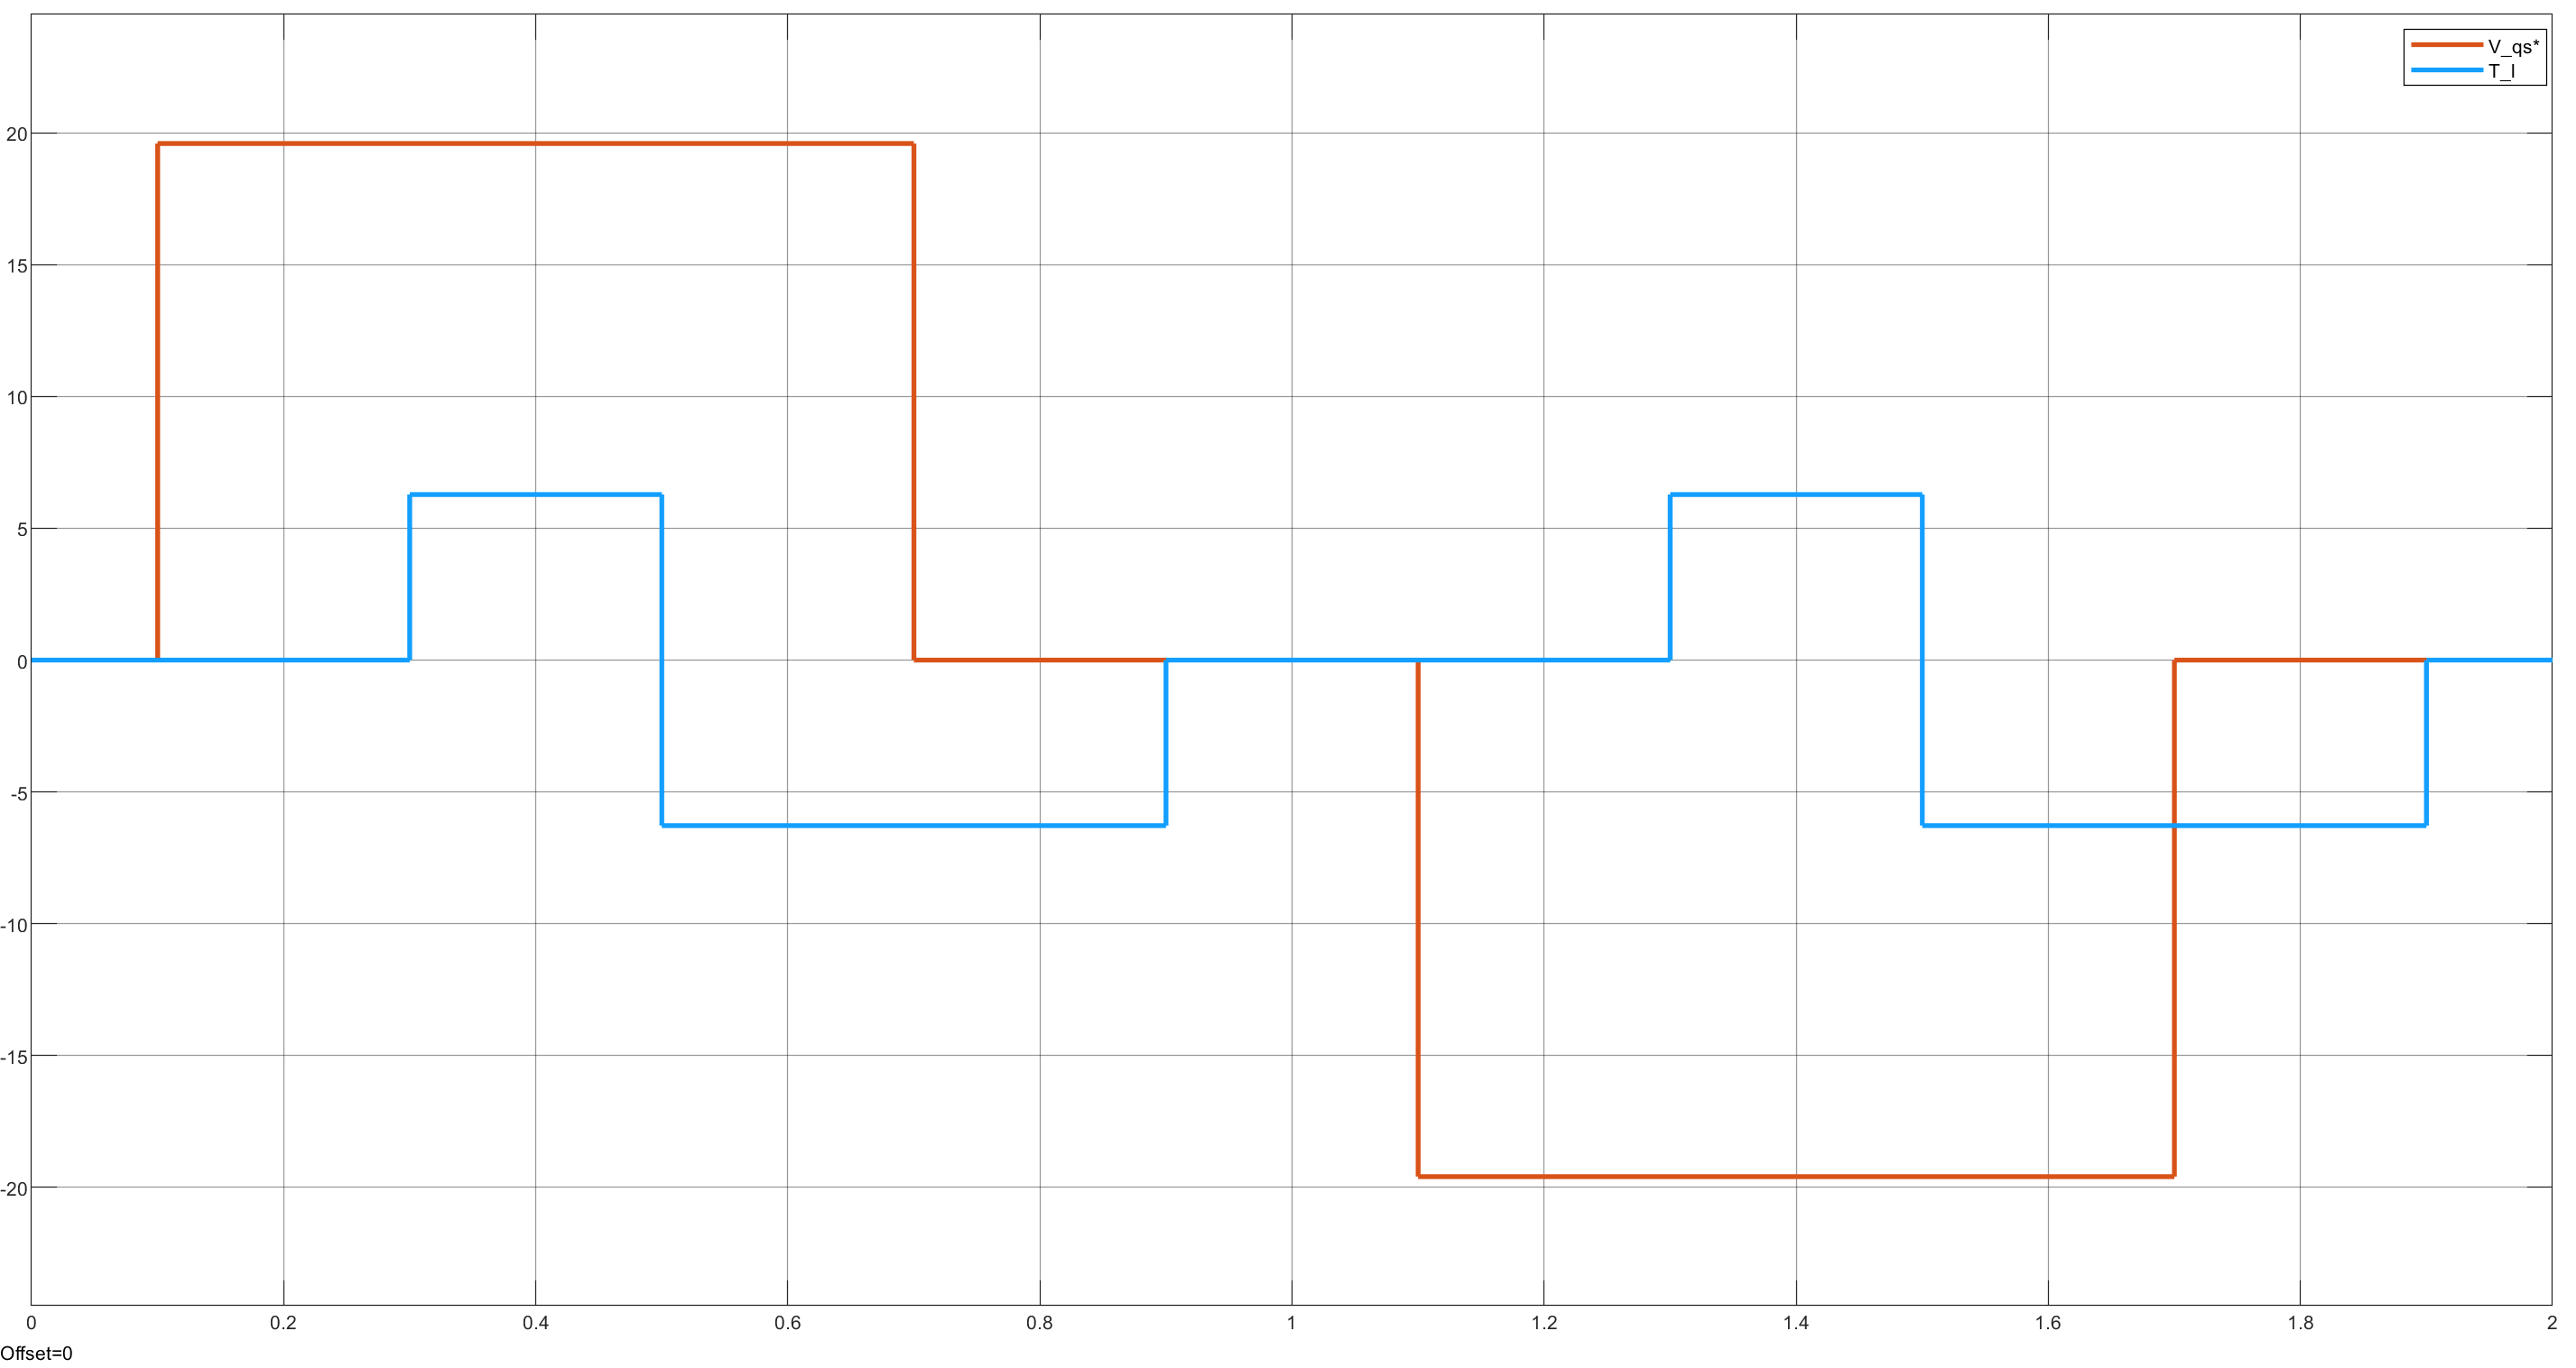
\includegraphics[width=\textwidth]{imagenes/sim_senales_entrada.png}
    \caption{Señales de excitación: consigna de tensión $v_{qs}^*(t)$ y torque de carga $T_{ld}(t)$.}
    \label{fig:sim_entradas}
\end{figure}

De la secuencia se identifican 10 transitorios consecutivos, separados por los instantes de conmutación $t_1 = 0{,}1$~s, $t_2 = 0{,}3$~s, $t_3 = 0{,}5$~s, $t_4 = 0{,}7$~s, $t_5 = 0{,}9$~s, $t_6 = 1{,}1$~s, $t_7 = 1{,}3$~s, $t_8 = 1{,}5$~s, $t_9 = 1{,}7$~s, $t_{10} = 1{,}9$~s. La primera mitad (Trans.~1--5) corresponde al pulso positivo de $v_{qs}^*$ y la segunda mitad (Trans.~6--10) a su simétrico negativo.

\subsubsection{Modelo en Simulink}

Se construyó un modelo en Simulink con dos subsistemas en paralelo: el modelo NL completo (implementado mediante \textit{MATLAB Function} con las 6 ecuaciones de estado y las leyes de control mínima y complementaria) y el modelo LTI aumentado (bloque \textit{State-Space} de 4 estados). Ambos reciben las mismas señales de excitación. La simulación también se reproduce con un script MATLAB (\texttt{simulacion\_dinamica\_516.m}) que utiliza \texttt{ode15s} para el modelo NL y \texttt{lsim} para el LTI, permitiendo post-procesamiento detallado.

\begin{figure}[H]
    \centering
    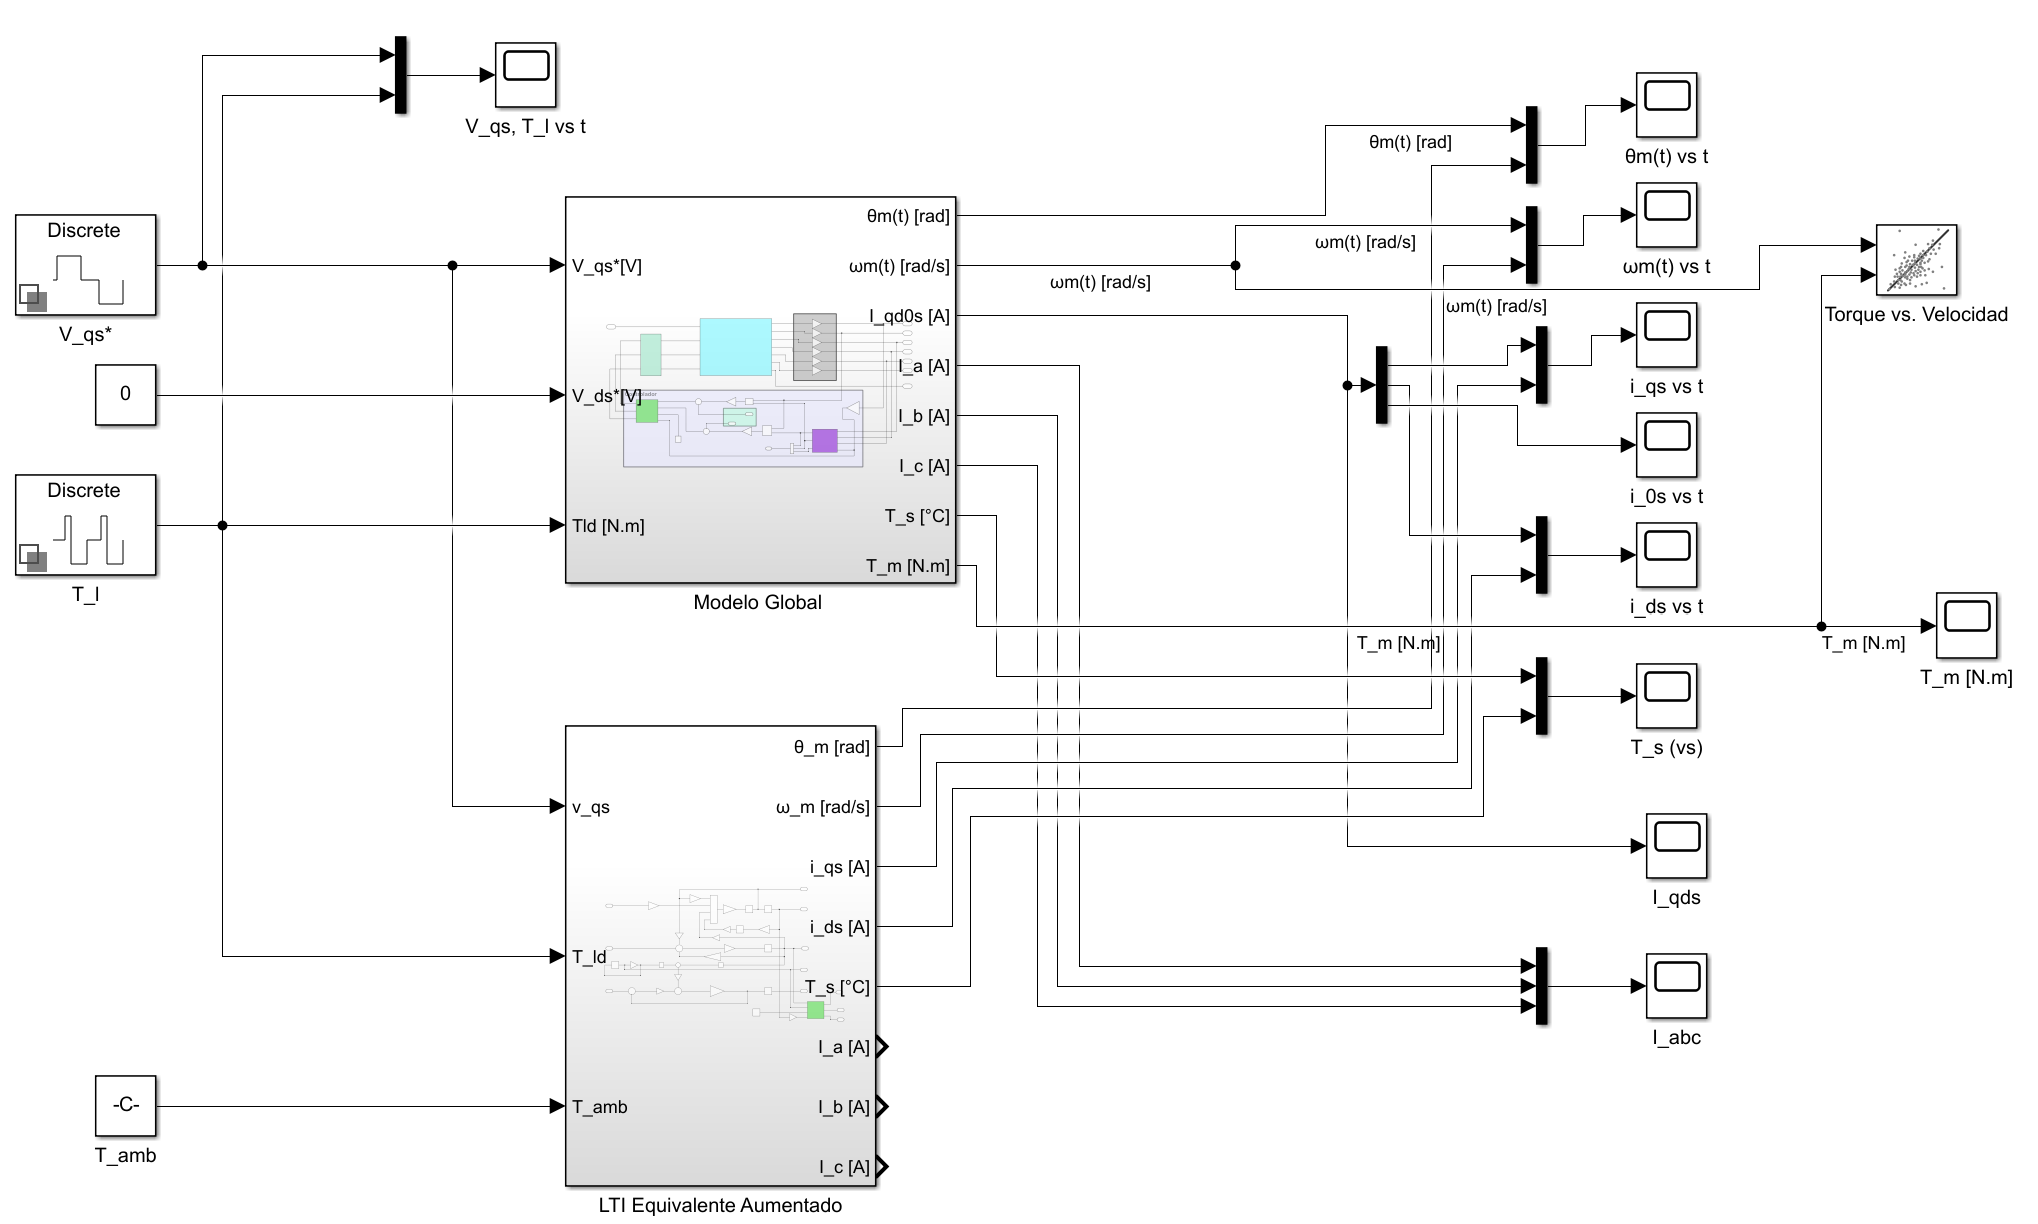
\includegraphics[width=\textwidth]{imagenes/sim_diagrama_bloques.png}
    \caption{Diagrama de bloques en Simulink: modelo NL desacoplado y LTI aumentado en paralelo.}
    \label{fig:simulink_diagrama}
\end{figure}

\subsubsection{Respuesta del estado interno (Sub-ítem a)}
\label{sec:sim_item_a}

Se presentan los resultados de la simulación para el caso nominal $i_{ds}^r(0) = 0$~A, comparando las salidas del modelo NL (6 estados) y del modelo LTI aumentado (4 estados) ante las mismas señales de excitación. Los efectos de $i_{ds}^r(0) \neq 0$ se analizan por separado en el Sub-ítem~c.

\paragraph{Posición angular $\theta_m(t)$.}

\begin{figure}[H]
    \centering
    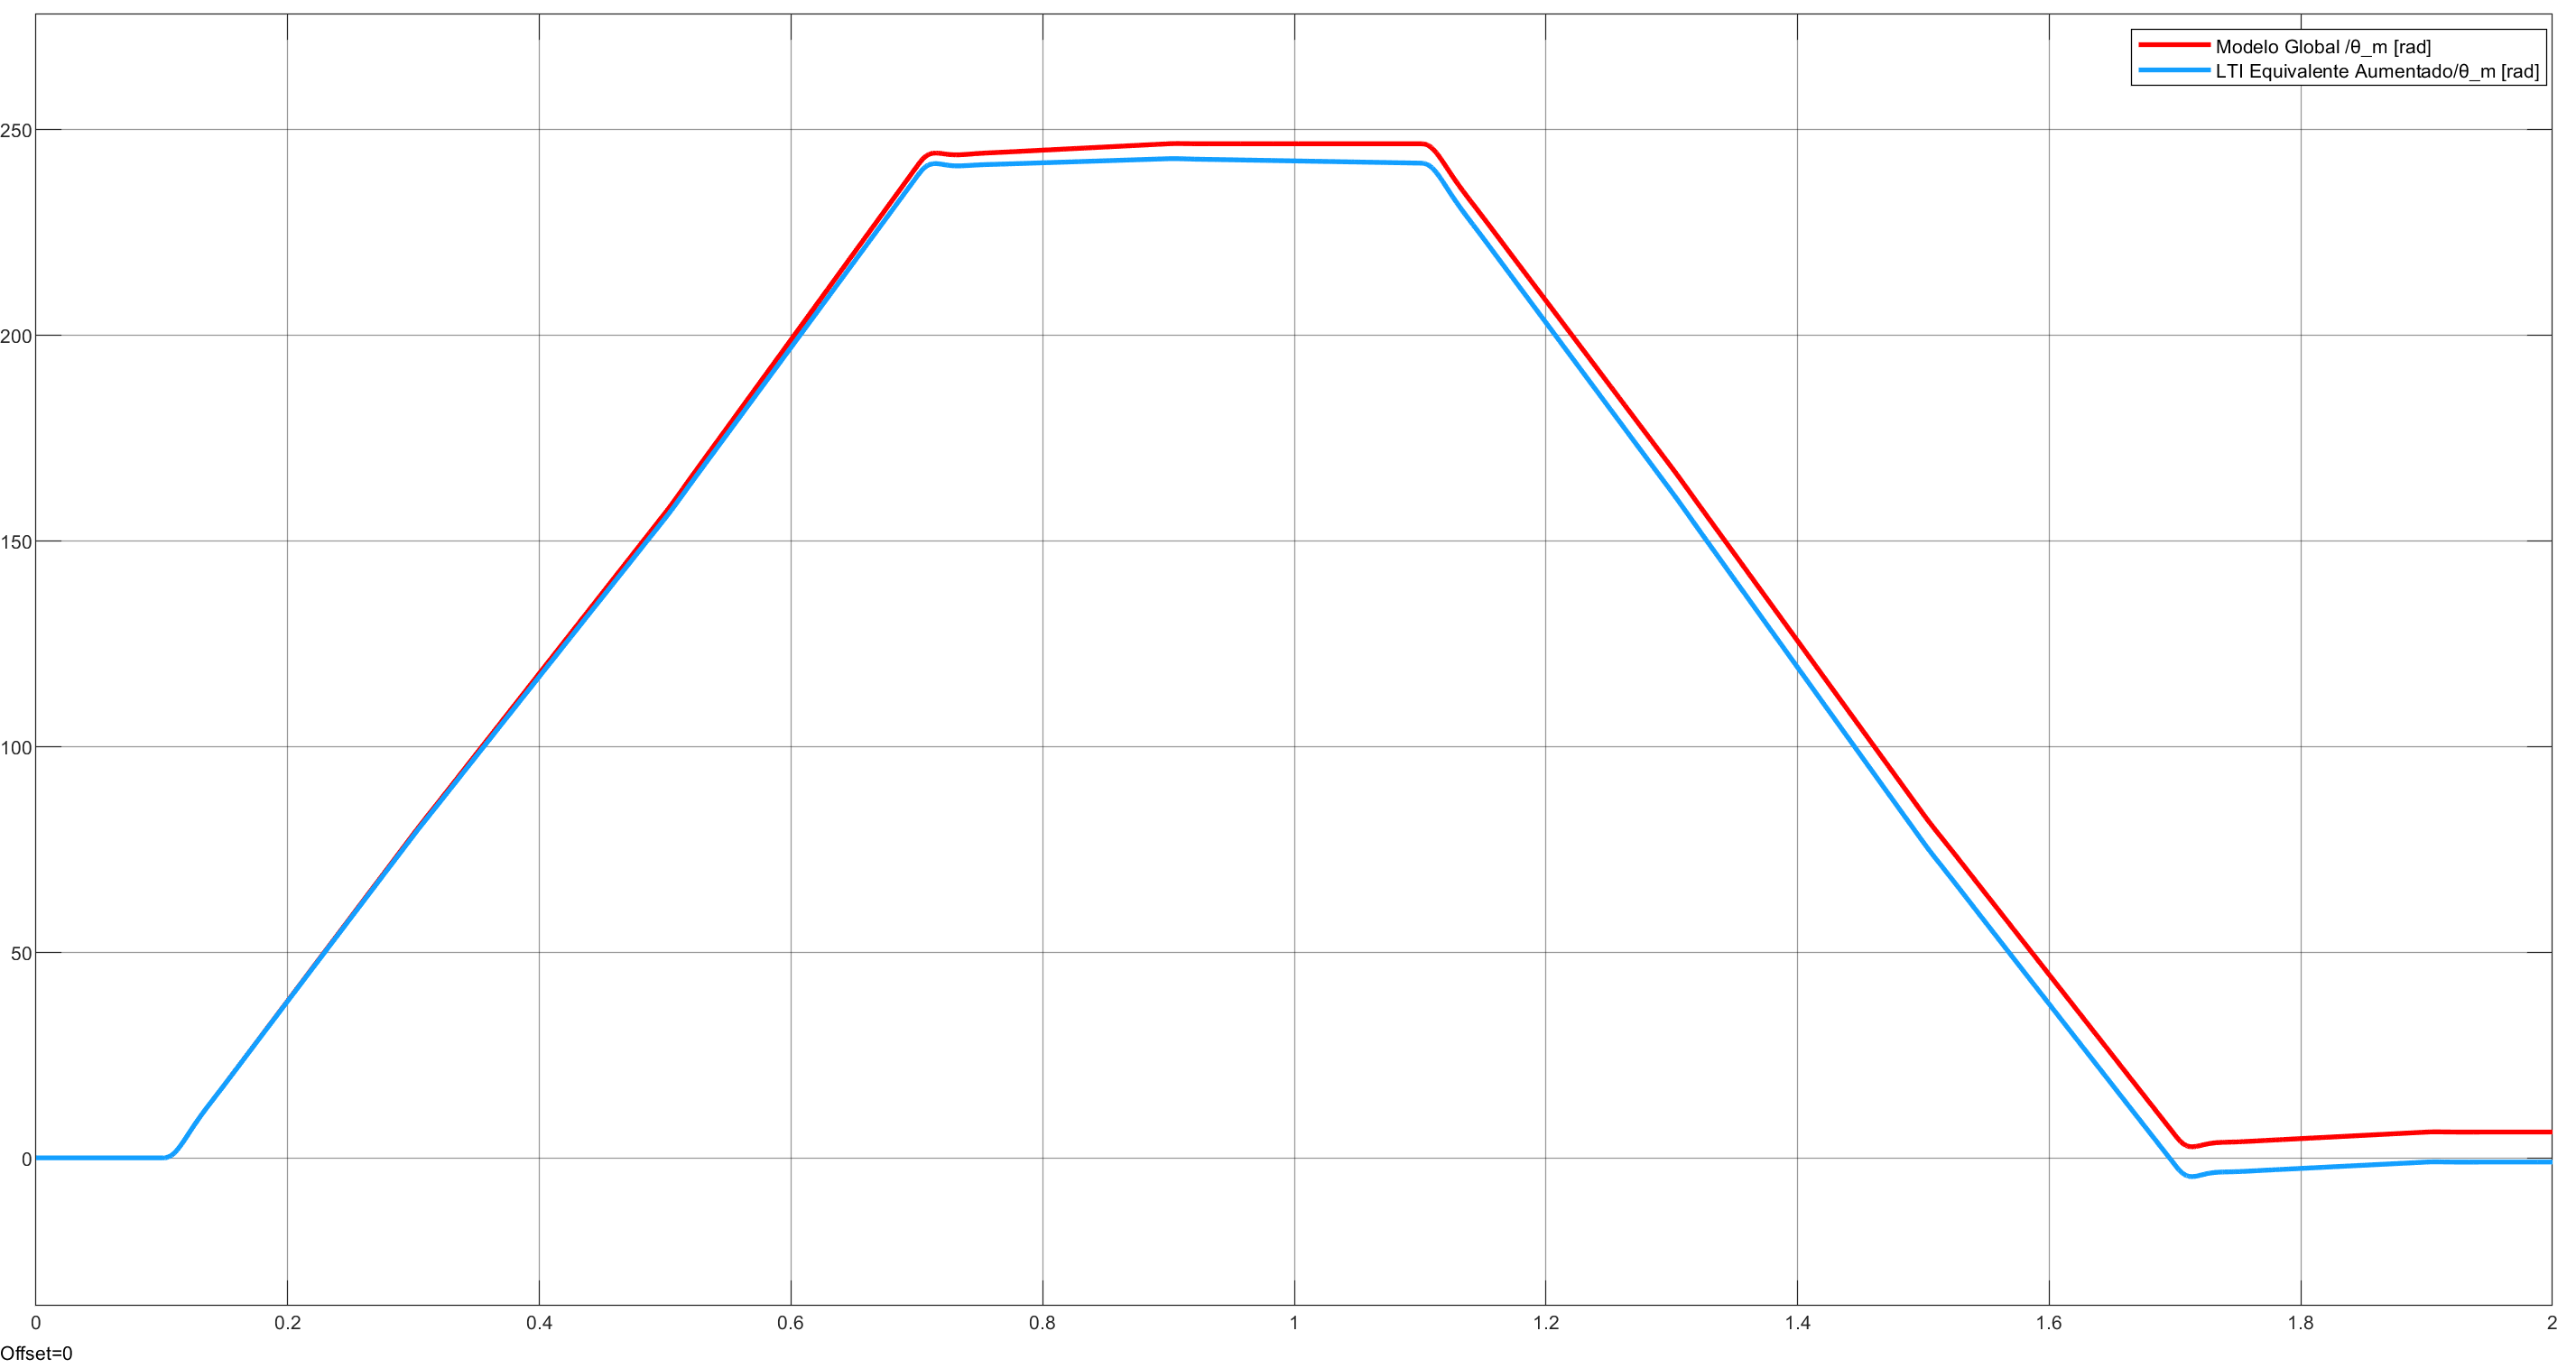
\includegraphics[width=\textwidth]{imagenes/sim_theta_m.png}
    \caption{Posición angular $\theta_m(t)$: comparación modelo NL vs LTI aumentado ($i_{ds}^r(0) = 0$~A).}
    \label{fig:sim_theta_m}
\end{figure}

La posición angular crece como rampa durante los pulsos de tensión, consecuencia directa del integrador puro ($\dot{\theta}_m = \omega_m$). Alcanza un máximo de $\approx 250$~rad en $t \approx 1$~s y retorna hacia cero durante el pulso negativo de $v_{qs}^*$. Ambos modelos presentan excelente concordancia. La pequeña diferencia residual al final (offset constante una vez que $\theta_m$ regresa cerca de cero) se debe a la acumulación del error integrado entre las velocidades de ambos modelos, efecto inherente a la presencia del integrador puro en la planta.

\paragraph{Velocidad angular $\omega_m(t)$.}

\begin{figure}[H]
    \centering
    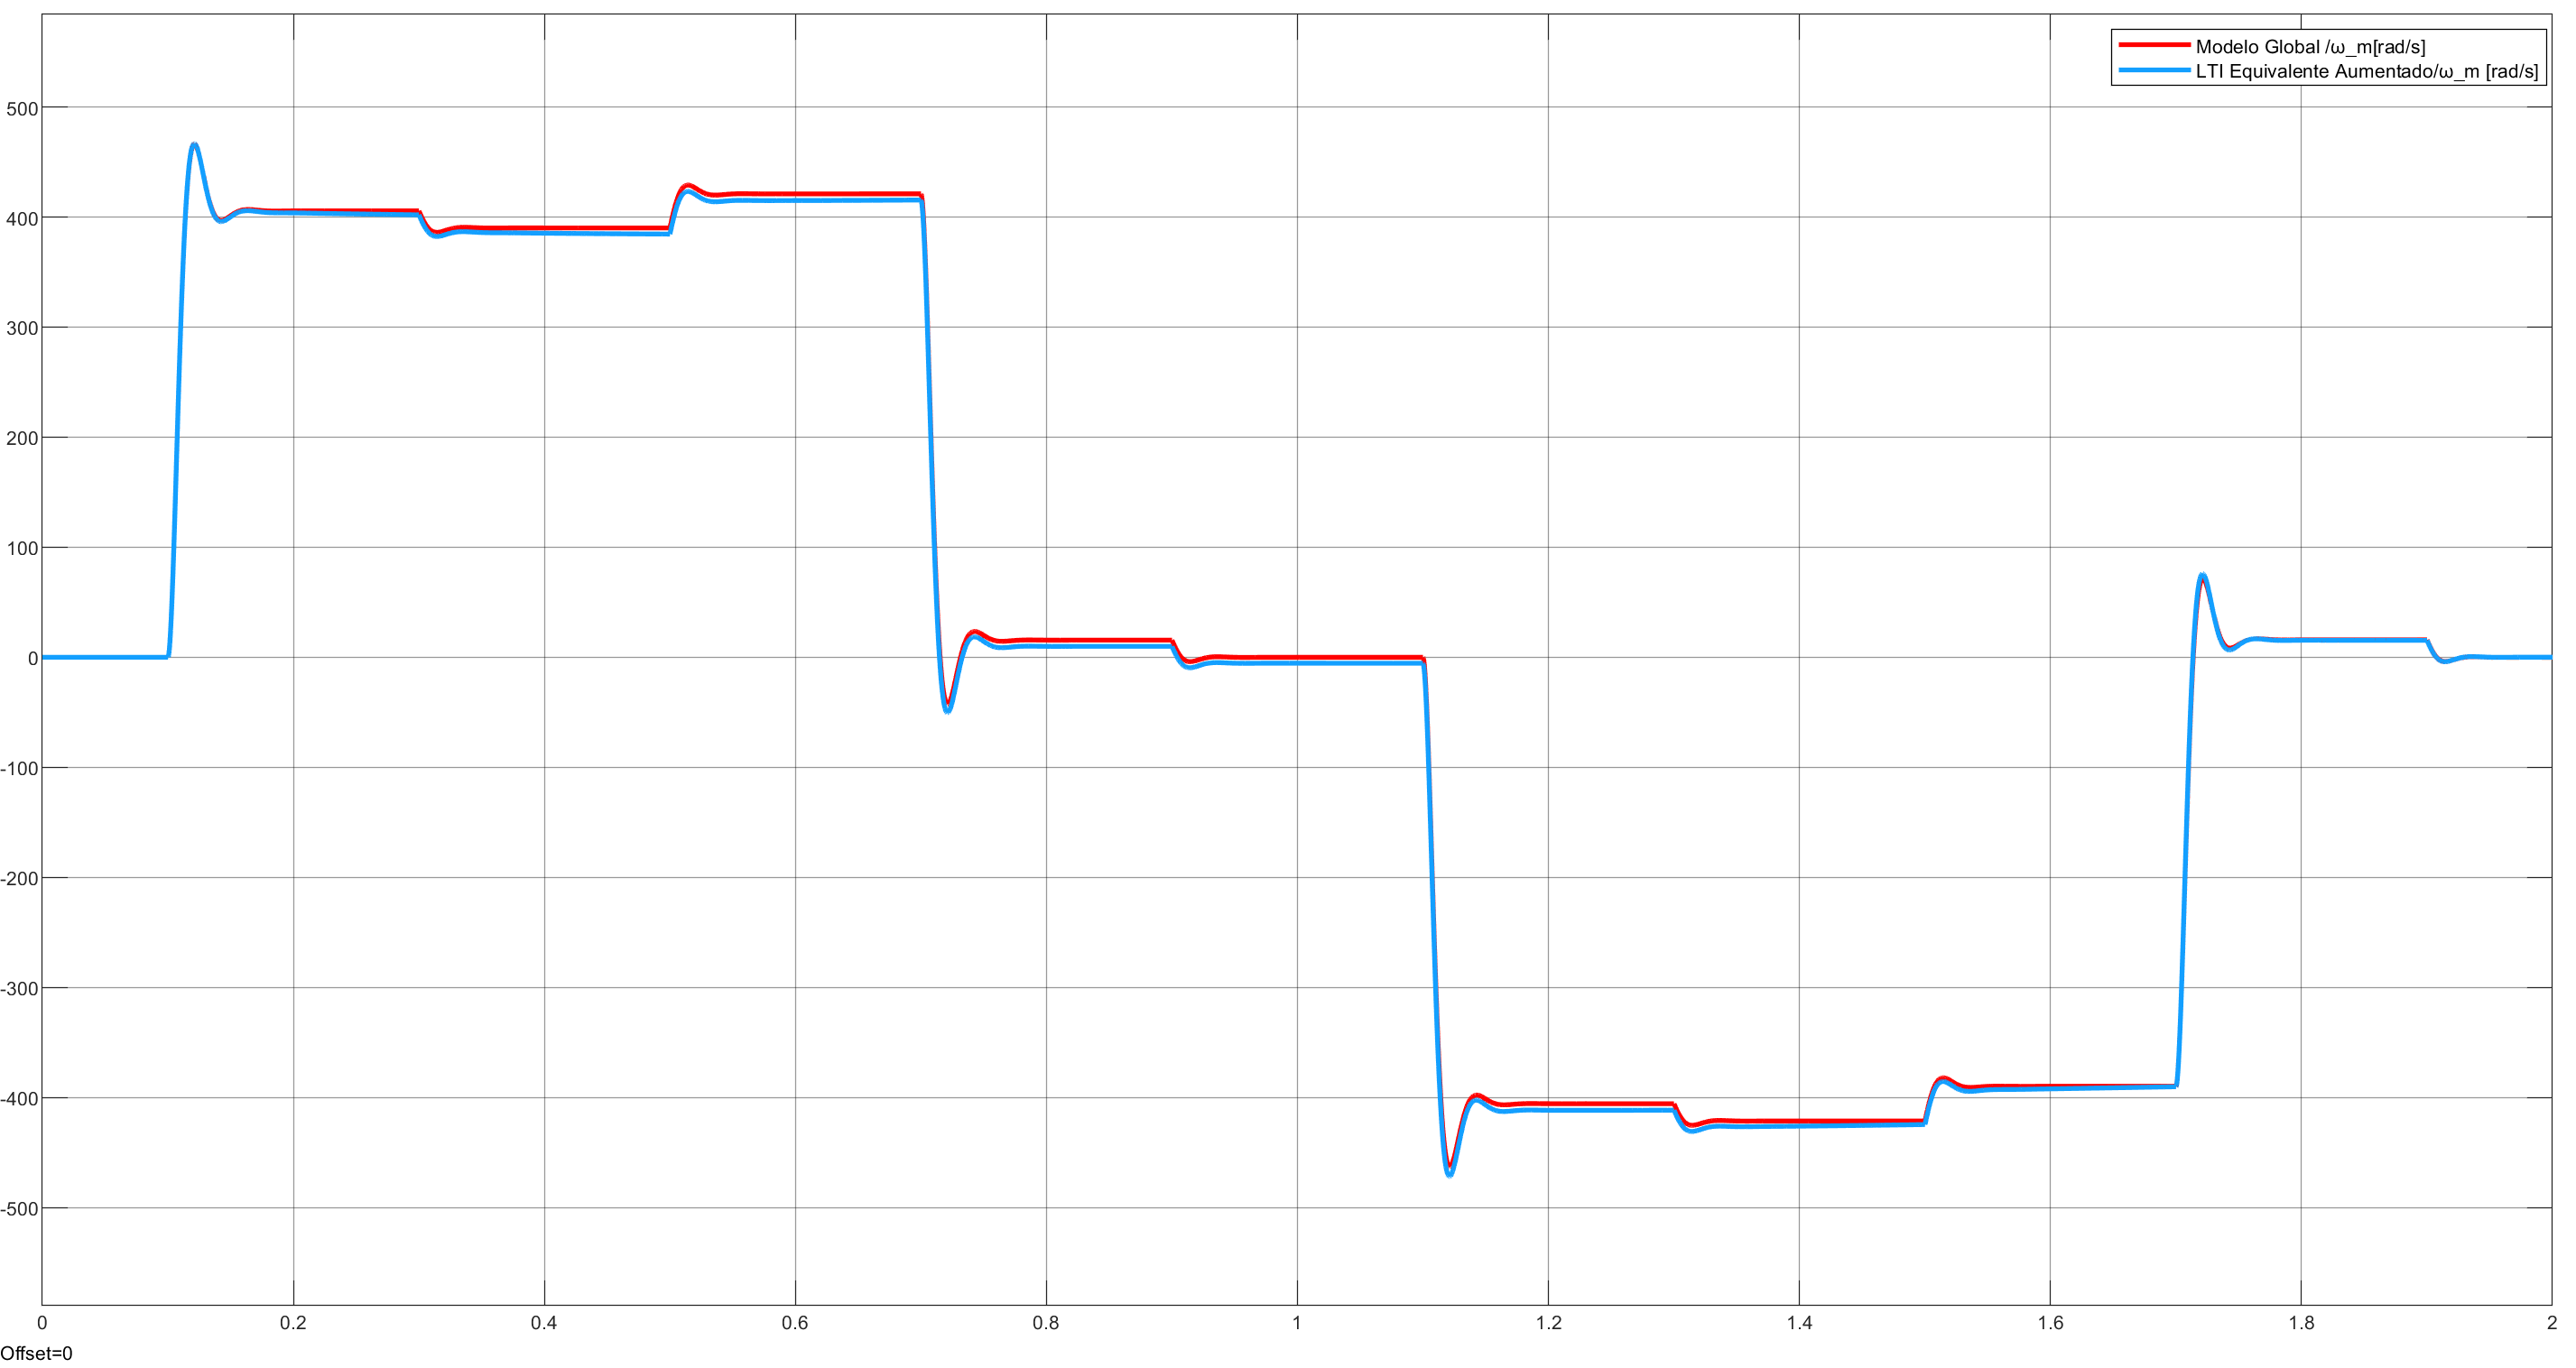
\includegraphics[width=\textwidth]{imagenes/sim_omega_m.png}
    \caption{Velocidad angular $\omega_m(t)$: comparación modelo NL vs LTI aumentado ($i_{ds}^r(0) = 0$~A).}
    \label{fig:sim_omega_m}
\end{figure}

La velocidad responde con dinámica dominada por la constante de tiempo mecánica $\tau_m = J_{eq}/b_{eq} \approx 0{,}70$~s. Durante el pulso positivo de $v_{qs}^*$ ($0{,}1$--$0{,}7$~s), $\omega_m$ crece hasta $\approx +400$~rad/s, modulada por las perturbaciones de torque de carga $T_{ld}$. Durante el pulso negativo ($1{,}1$--$1{,}7$~s), la respuesta es simétrica, alcanzando $\approx -400$~rad/s. La concordancia NL--LTI es excelente, confirmando la efectividad de la linealización por retroalimentación NL.

\paragraph{Corriente $i_{qs}(t)$.}

\begin{figure}[H]
    \centering
    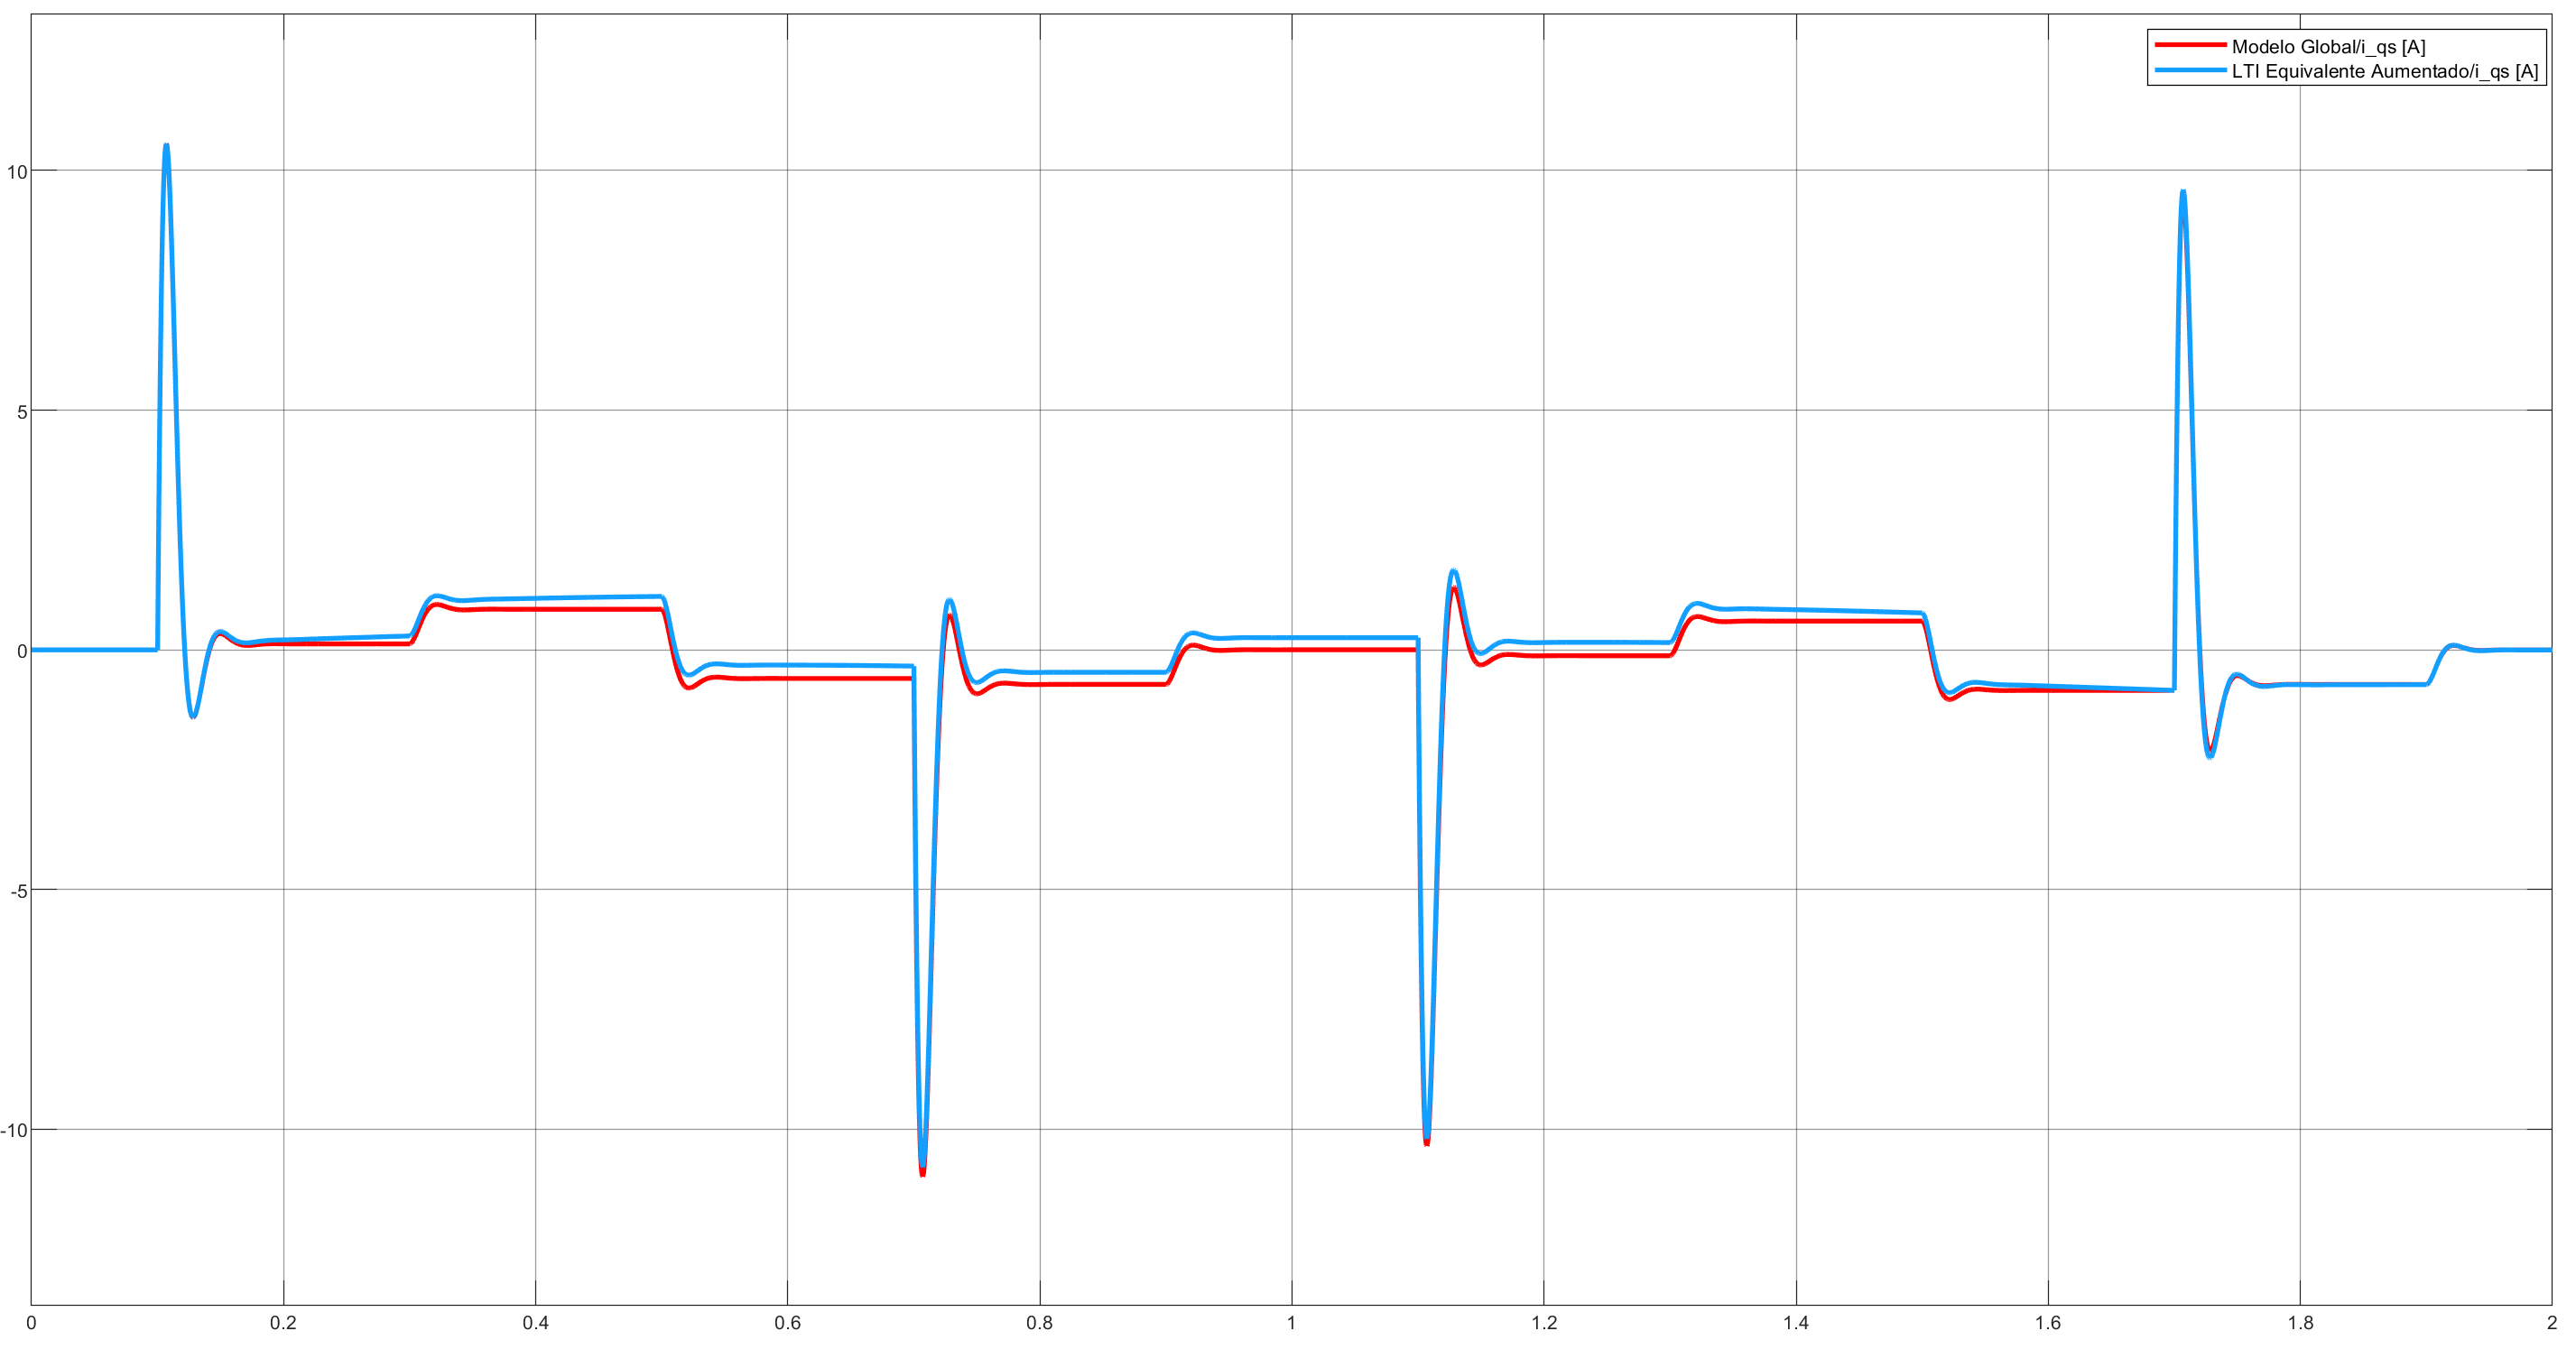
\includegraphics[width=\textwidth]{imagenes/sim_iqs.png}
    \caption{Corriente de eje $q$, $i_{qs}(t)$: comparación modelo NL vs LTI aumentado ($i_{ds}^r(0) = 0$~A).}
    \label{fig:sim_iqs}
\end{figure}

La corriente $i_{qs}$ responde rápidamente a los escalones de $v_{qs}^*$ con constante de tiempo eléctrica $\tau_e = L_q/R_{s0} \approx 5{,}69$~ms, alcanzando su valor de régimen en $\approx 5\tau_e \approx 28{,}4$~ms. Se observan picos de $\approx \pm 10$~A. Ambos modelos se solapan casi perfectamente, confirmando que las leyes de control NL linealizan efectivamente el sistema. Dado que para $i_{ds}^r = 0$ el torque electromagnético se reduce a $T_{em} = k_t \cdot i_{qs}$ (con $k_t = \tfrac{3}{2} P_p \lambda_r$), la forma de onda de $T_{em}(t)$ es directamente proporcional a $i_{qs}(t)$.

\paragraph{Corrientes $i_{ds}(t)$ e $i_{0s}(t)$.} Para la condición inicial $i_{ds}^r(0) = 0$~A, la corriente de eje $d$ permanece idénticamente nula en ambos modelos durante toda la simulación, ya que no existe excitación externa en el eje $d$ ($v_{ds}^* = 0$) y la ley de control mínima ($v_{ds} = -L_q i_{qs} \omega_r$) compensa exactamente el acoplamiento cruzado sin inyectar corriente en dicho eje. Análogamente, la corriente de secuencia cero $i_{0s}(t)$ permanece nula al no existir excitación homopolar ($v_{0s} = 0$) ni condición inicial no nula. El comportamiento de $i_{ds}^r(t)$ para condiciones iniciales $i_{ds}^r(0) \neq 0$ se analiza en detalle en el Sub-ítem~c.

\paragraph{Temperatura del estator $T_s(t)$.}

\begin{figure}[H]
    \centering
    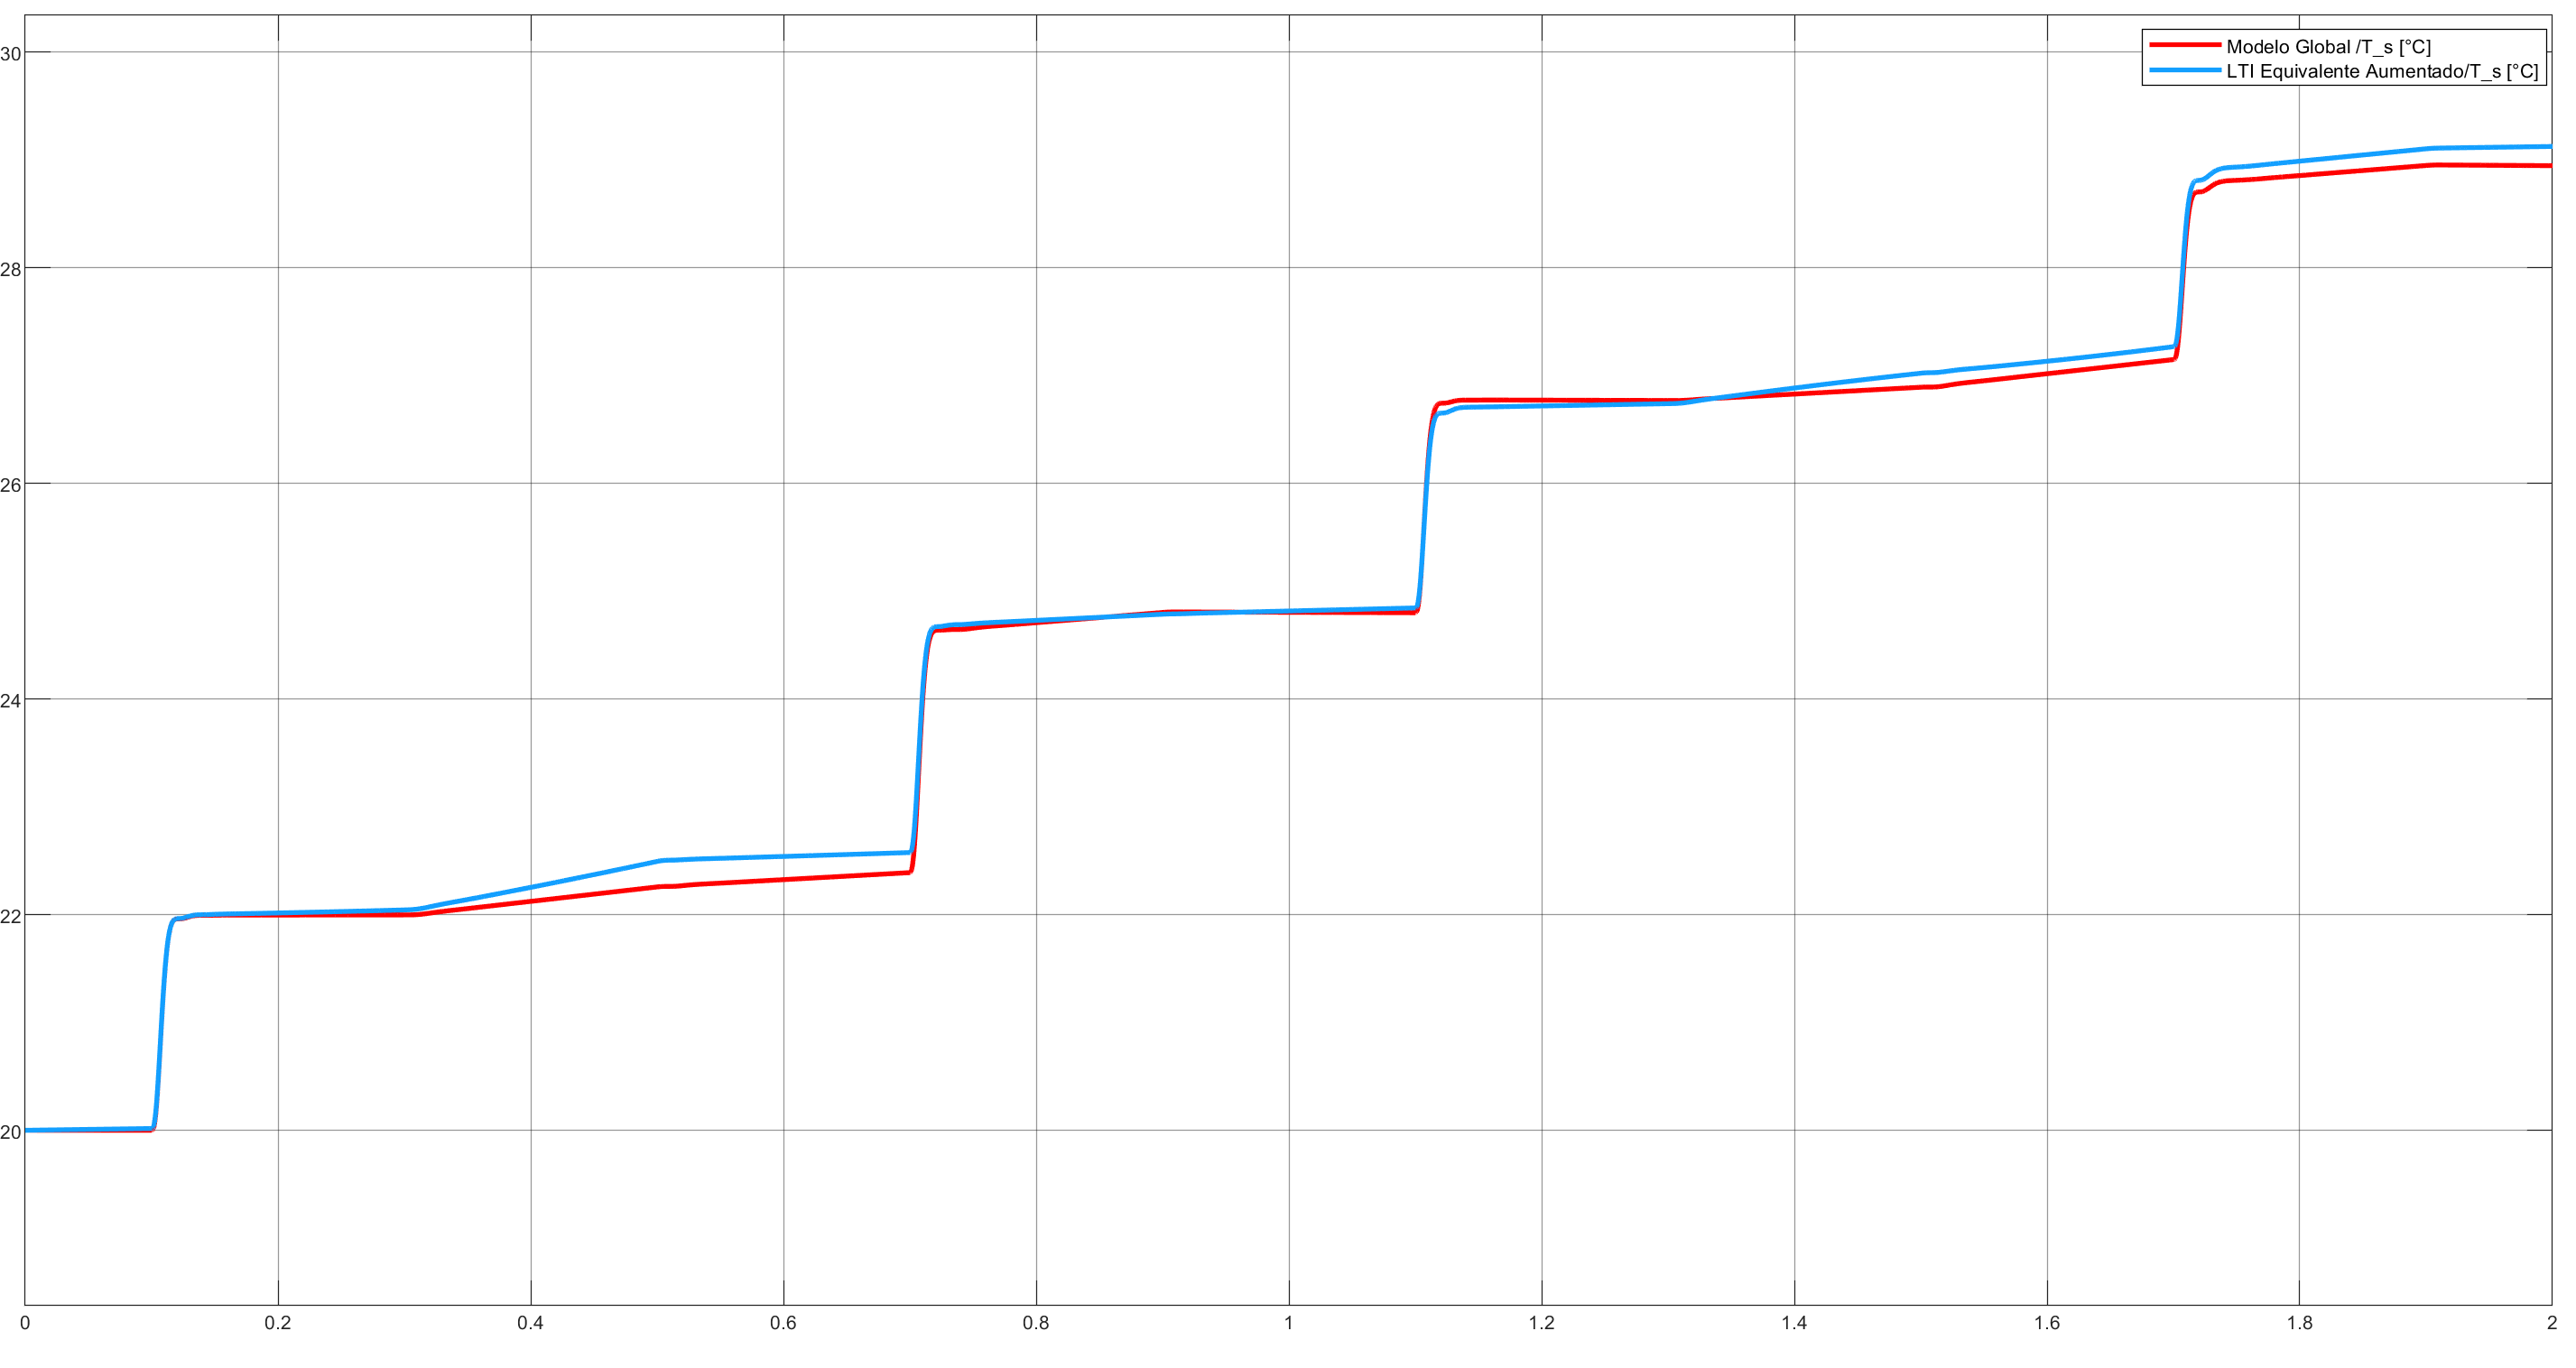
\includegraphics[width=\textwidth]{imagenes/sim_Ts.png}
    \caption{Temperatura del estator $T_s(t)$ del modelo NL ($i_{ds}^r(0) = 0$~A). El modelo LTI no incluye $T_s$ como variable de estado.}
    \label{fig:sim_Ts}
\end{figure}

La temperatura crece levemente respecto de $T_{amb} = 20\,^\circ$C debido a las pérdidas resistivas $P_{Cu} = \tfrac{3}{2}R_s(i_{qs}^2 + i_{ds}^{r\,2})$. El cambio es mínimo dado que la constante de tiempo térmica $\tau_{th} = R_{ts\text{-}amb} \cdot C_{ts} \approx 120$~s es muy superior a la duración de la simulación ($2{,}2$~s). Este resultado justifica la hipótesis del modelo LTI de utilizar $R_s = R_{sREF}$ constante: la variación de resistencia por efecto térmico es despreciable en esta escala temporal. Nótese que el modelo LTI aumentado (4 estados) \textbf{no incluye} la temperatura como variable de estado, ya que asume $R_s$ constante por diseño.

\paragraph{Tensión $v_{ds}(t)$ de la ley de control mínima.} La ley de control mínima impone internamente la tensión $v_{ds} = -L_q \, i_{qs} \, \omega_r$, proporcional al producto $i_{qs} \cdot \omega_m$. Esta tensión es no nula solo cuando ambas variables lo son simultáneamente, y su magnitud crece con el nivel de operación del sistema. Al ser una variable interna del modelo NL (no disponible como salida directa en la implementación Simulink actual), no se presenta su gráfico, pero su efecto se evidencia en la concordancia entre modelos: es precisamente esta ley la que desacopla los ejes $q$ y $d$, permitiendo que el modelo NL se comporte como el LTI.

\paragraph{Corrientes en coordenadas $abc$.} Mediante la transformada inversa de Park se obtienen las corrientes de fase reales que circularían por los bobinados del estator:
\begin{equation}
    \begin{bmatrix} i_a \\ i_b \\ i_c \end{bmatrix} = \mathbf{T}_{dq0}^{-1}(\theta_e) \begin{bmatrix} i_{ds}^r \\ i_{qs} \\ i_{0s} \end{bmatrix}, \quad \theta_e = P_p \cdot \theta_m
\end{equation}

\begin{figure}[H]
    \centering
    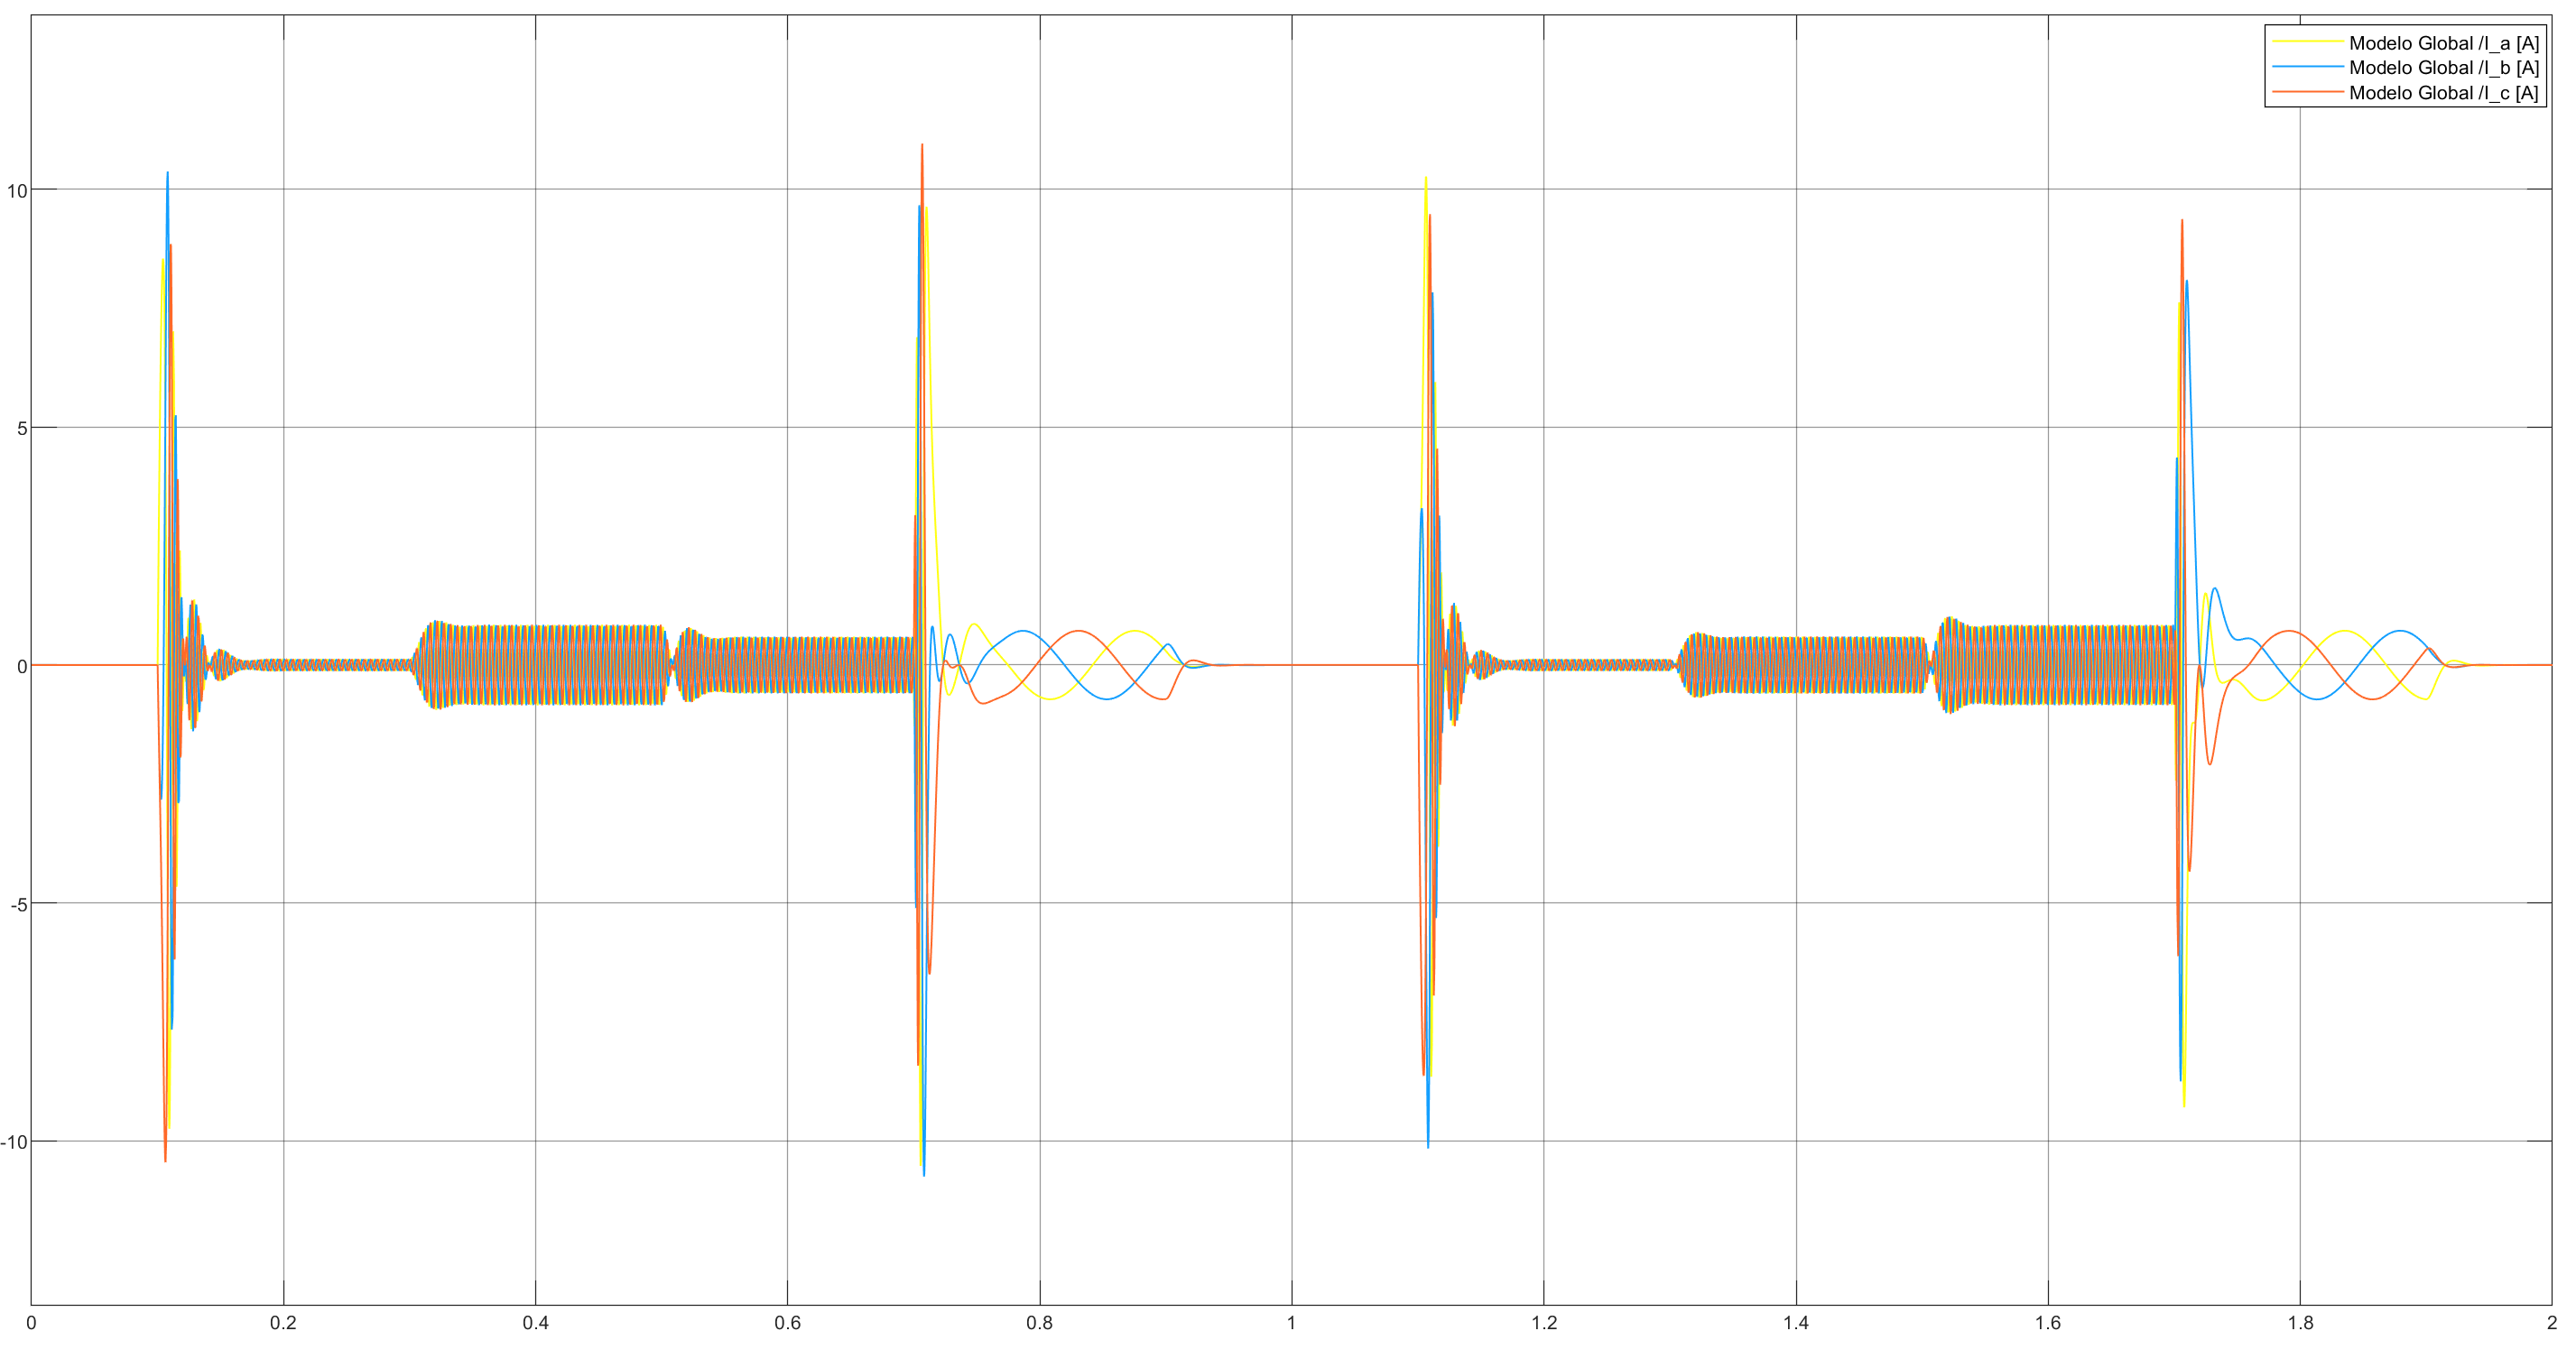
\includegraphics[width=\textwidth]{imagenes/sim_corrientes_abc.png}
    \caption{Corrientes de fase $i_a$, $i_b$, $i_c$ obtenidas por transformada inversa de Park (modelo NL, $i_{ds}^r(0) = 0$~A).}
    \label{fig:sim_corrientes_abc}
\end{figure}

Las formas de onda resultantes son sinusoidales moduladas en amplitud, con frecuencia eléctrica $\omega_e = P_p \cdot \omega_m$ proporcional a la velocidad del rotor. Cuando $\omega_m = 0$ (antes de $t = 0{,}1$~s y en los intervalos de velocidad nula), las corrientes $abc$ son constantes (frecuencia eléctrica nula). A medida que el motor acelera, la frecuencia de las oscilaciones crece proporcionalmente.

\paragraph{Curva paramétrica: torque vs velocidad (cuadrantes de operación).}

La curva paramétrica $T_{em}(\omega_m)$ se construye a partir de los datos del script MATLAB, segmentando la trayectoria en 10 transitorios que conectan los puntos de (cuasi-)equilibrio $P_0$ a $P_{10}$.

\begin{figure}[H]
    \centering
    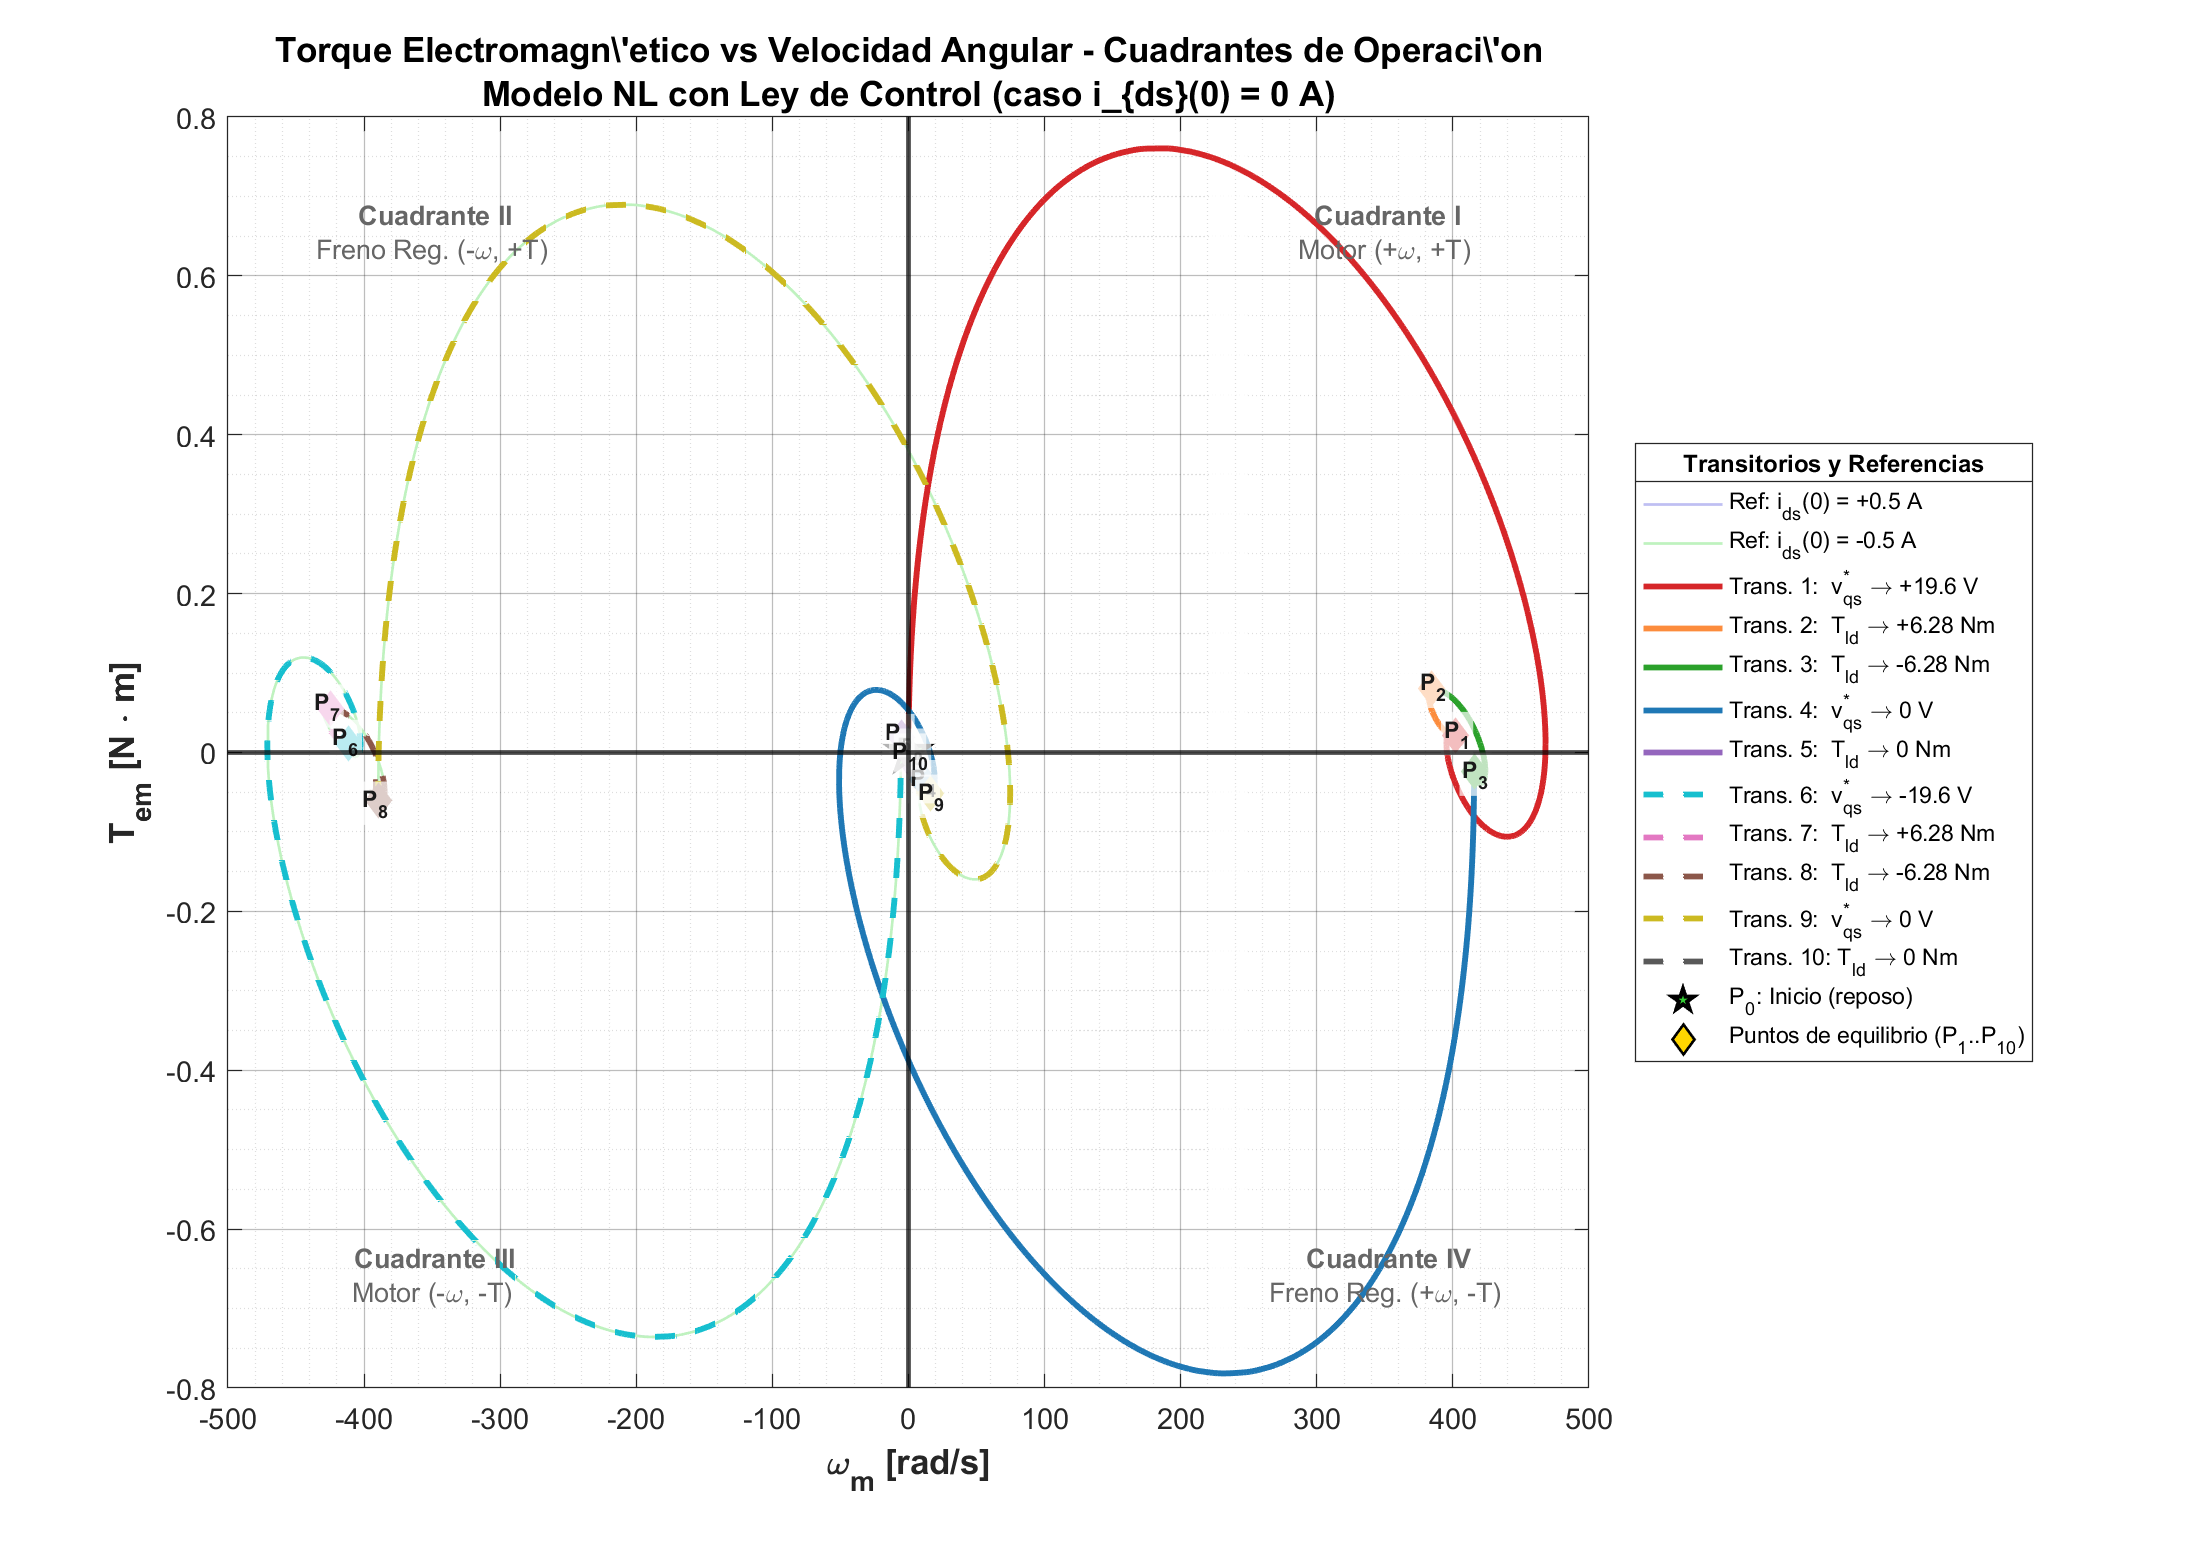
\includegraphics[width=\textwidth]{imagenes/sim_torque_vs_velocidad.png}
    \caption{Torque electromagnético vs velocidad angular: cuadrantes de operación del motor PMSM. Cada transitorio se distingue por color, con flechas indicando el sentido de recorrido y diamantes marcando los puntos de equilibrio $P_0$ a $P_{10}$.}
    \label{fig:sim_torque_vel}
\end{figure}

El sistema recorre los cuatro cuadrantes durante la secuencia completa de pulsos:
\begin{itemize}
    \item \textbf{Cuadrante I} ($+\omega_m, +T_{em}$): motorización en sentido positivo. El motor entrega torque en el mismo sentido que la velocidad.
    \item \textbf{Cuadrante II} ($-\omega_m, +T_{em}$): frenado regenerativo en sentido negativo.
    \item \textbf{Cuadrante III} ($-\omega_m, -T_{em}$): motorización en sentido negativo, análogo al Cuadrante~I para el pulso negativo de $v_{qs}^*$.
    \item \textbf{Cuadrante IV} ($+\omega_m, -T_{em}$): frenado regenerativo en sentido positivo. El torque frena la velocidad positiva residual.
\end{itemize}

\paragraph{Plano de corrientes $i_{ds}^r$ vs $i_{qs}$ y ángulo de torque.} Para $i_{ds}^r(0) = 0$, la trayectoria en el plano $(i_{qs},\, i_{ds}^r)$ permanece sobre el eje $i_{qs}$ durante toda la simulación, correspondiendo al control vectorial ideal donde todo el vector de corriente se alinea con el eje $q$. El ángulo de torque $\delta = \text{atan2}(i_{ds}^r, i_{qs})$ resulta $\delta \equiv 0°$, confirmando la condición óptima que maximiza la relación torque/corriente. Las trayectorias en este plano y la evolución de $\delta(t)$ para $i_{ds}^r(0) \neq 0$ se presentan en el Sub-ítem~c, donde la comparación resulta visualmente más informativa.

% =====================================================================
\subsubsection{Métricas de transitorio (Sub-ítem b)}
\label{sec:sim_item_b}

Se determinan las métricas de los 10 transitorios para el caso nominal $i_{ds}^r(0) = 0$~A del modelo LTI. La Tabla~\ref{tab:metricas_trans} resume los valores finales de establecimiento, tiempos de crecimiento (10\,\% al 90\,\%), tiempos de asentamiento ($\pm 1$\,\%) y sobrepico para la velocidad angular $\omega_m$ y la corriente $i_{qs}$.

\begin{table}[H]
    \centering
    \caption{Métricas de transitorio para cada evento de conmutación (modelo LTI, $i_{ds}^r(0) = 0$~A).}
    \label{tab:metricas_trans}
    \renewcommand{\arraystretch}{1.15}
    \footnotesize
    \begin{tabular}{|c|c|c|c|c|c|c|}
        \hline
        \textbf{Trans.} & \textbf{Evento} & $\omega_{m,ss}$ & $i_{qs,ss}$ & $t_r$ & $t_s$ & $M_p$ \\
         & & [rad/s] & [A] & [ms] & [ms] & [\%] \\
        \hline
        1 & $v_{qs}^* \to +19{,}6$~V & -- & -- & -- & -- & -- \\
        2 & $T_{ld} \to +6{,}28$~Nm & -- & -- & -- & -- & -- \\
        3 & $T_{ld} \to -6{,}28$~Nm & -- & -- & -- & -- & -- \\
        4 & $v_{qs}^* \to 0$~V & -- & -- & -- & -- & -- \\
        5 & $T_{ld} \to 0$~Nm & -- & -- & -- & -- & -- \\
        6 & $v_{qs}^* \to -19{,}6$~V & -- & -- & -- & -- & -- \\
        7 & $T_{ld} \to +6{,}28$~Nm & -- & -- & -- & -- & -- \\
        8 & $T_{ld} \to -6{,}28$~Nm & -- & -- & -- & -- & -- \\
        9 & $v_{qs}^* \to 0$~V & -- & -- & -- & -- & -- \\
        10 & $T_{ld} \to 0$~Nm & -- & -- & -- & -- & -- \\
        \hline
    \end{tabular}

    \vspace{2mm}
    \scriptsize Nota: completar con valores numéricos de la simulación MATLAB.
\end{table}

\textbf{Influencia relativa de las acciones externas:}

\begin{itemize}
    \item \textbf{Tensión $v_{qs}^*(t)$}: actúa directamente sobre la corriente $i_{qs}$ a través de la dinámica eléctrica rápida ($\tau_e = L_q/R_{s0} = 5{,}69$~ms). Es la acción \textbf{dominante} porque genera el torque electromagnético $T_{em} = k_t \cdot i_{qs}$, que a su vez impulsa la dinámica mecánica. El efecto sobre $\omega_m$ es indirecto pero determinante (pasa por el integrador mecánico).

    \item \textbf{Torque de carga $T_{ld}(t)$}: actúa \textbf{directamente} sobre la velocidad $\omega_m$ a través de la ecuación mecánica, con constante de tiempo $\tau_m = J_{eq}/b_{eq} \approx 0{,}70$~s. Es una perturbación que modifica el punto de equilibrio de velocidad sin alterar la corriente $i_{qs}$ (que depende solo de $v_{qs}^*$).

    \item La separación de escalas temporales ($\tau_e \ll \tau_m$, ratio $\approx 1:123$) explica por qué las corrientes responden casi instantáneamente a cambios de tensión, mientras que la velocidad presenta transitorios mucho más lentos. Los cambios en $T_{ld}$ se manifiestan como escalones en $\omega_{m,ss}$ sin sobrepico apreciable.
\end{itemize}

% =====================================================================
\subsubsection{Efecto de $i_{ds}^r(0)$ sobre el sistema (Sub-ítem c)}
\label{sec:sim_item_c}

Se compara el comportamiento de $i_{ds}^r(t)$ para las tres condiciones iniciales en ambos modelos.

% TODO Paso 2: descomentar cuando se tengan las imágenes de las 3 corridas con i_ds(0) = 0, +0.5, -0.5
%\begin{figure}[H]
%    \centering
%    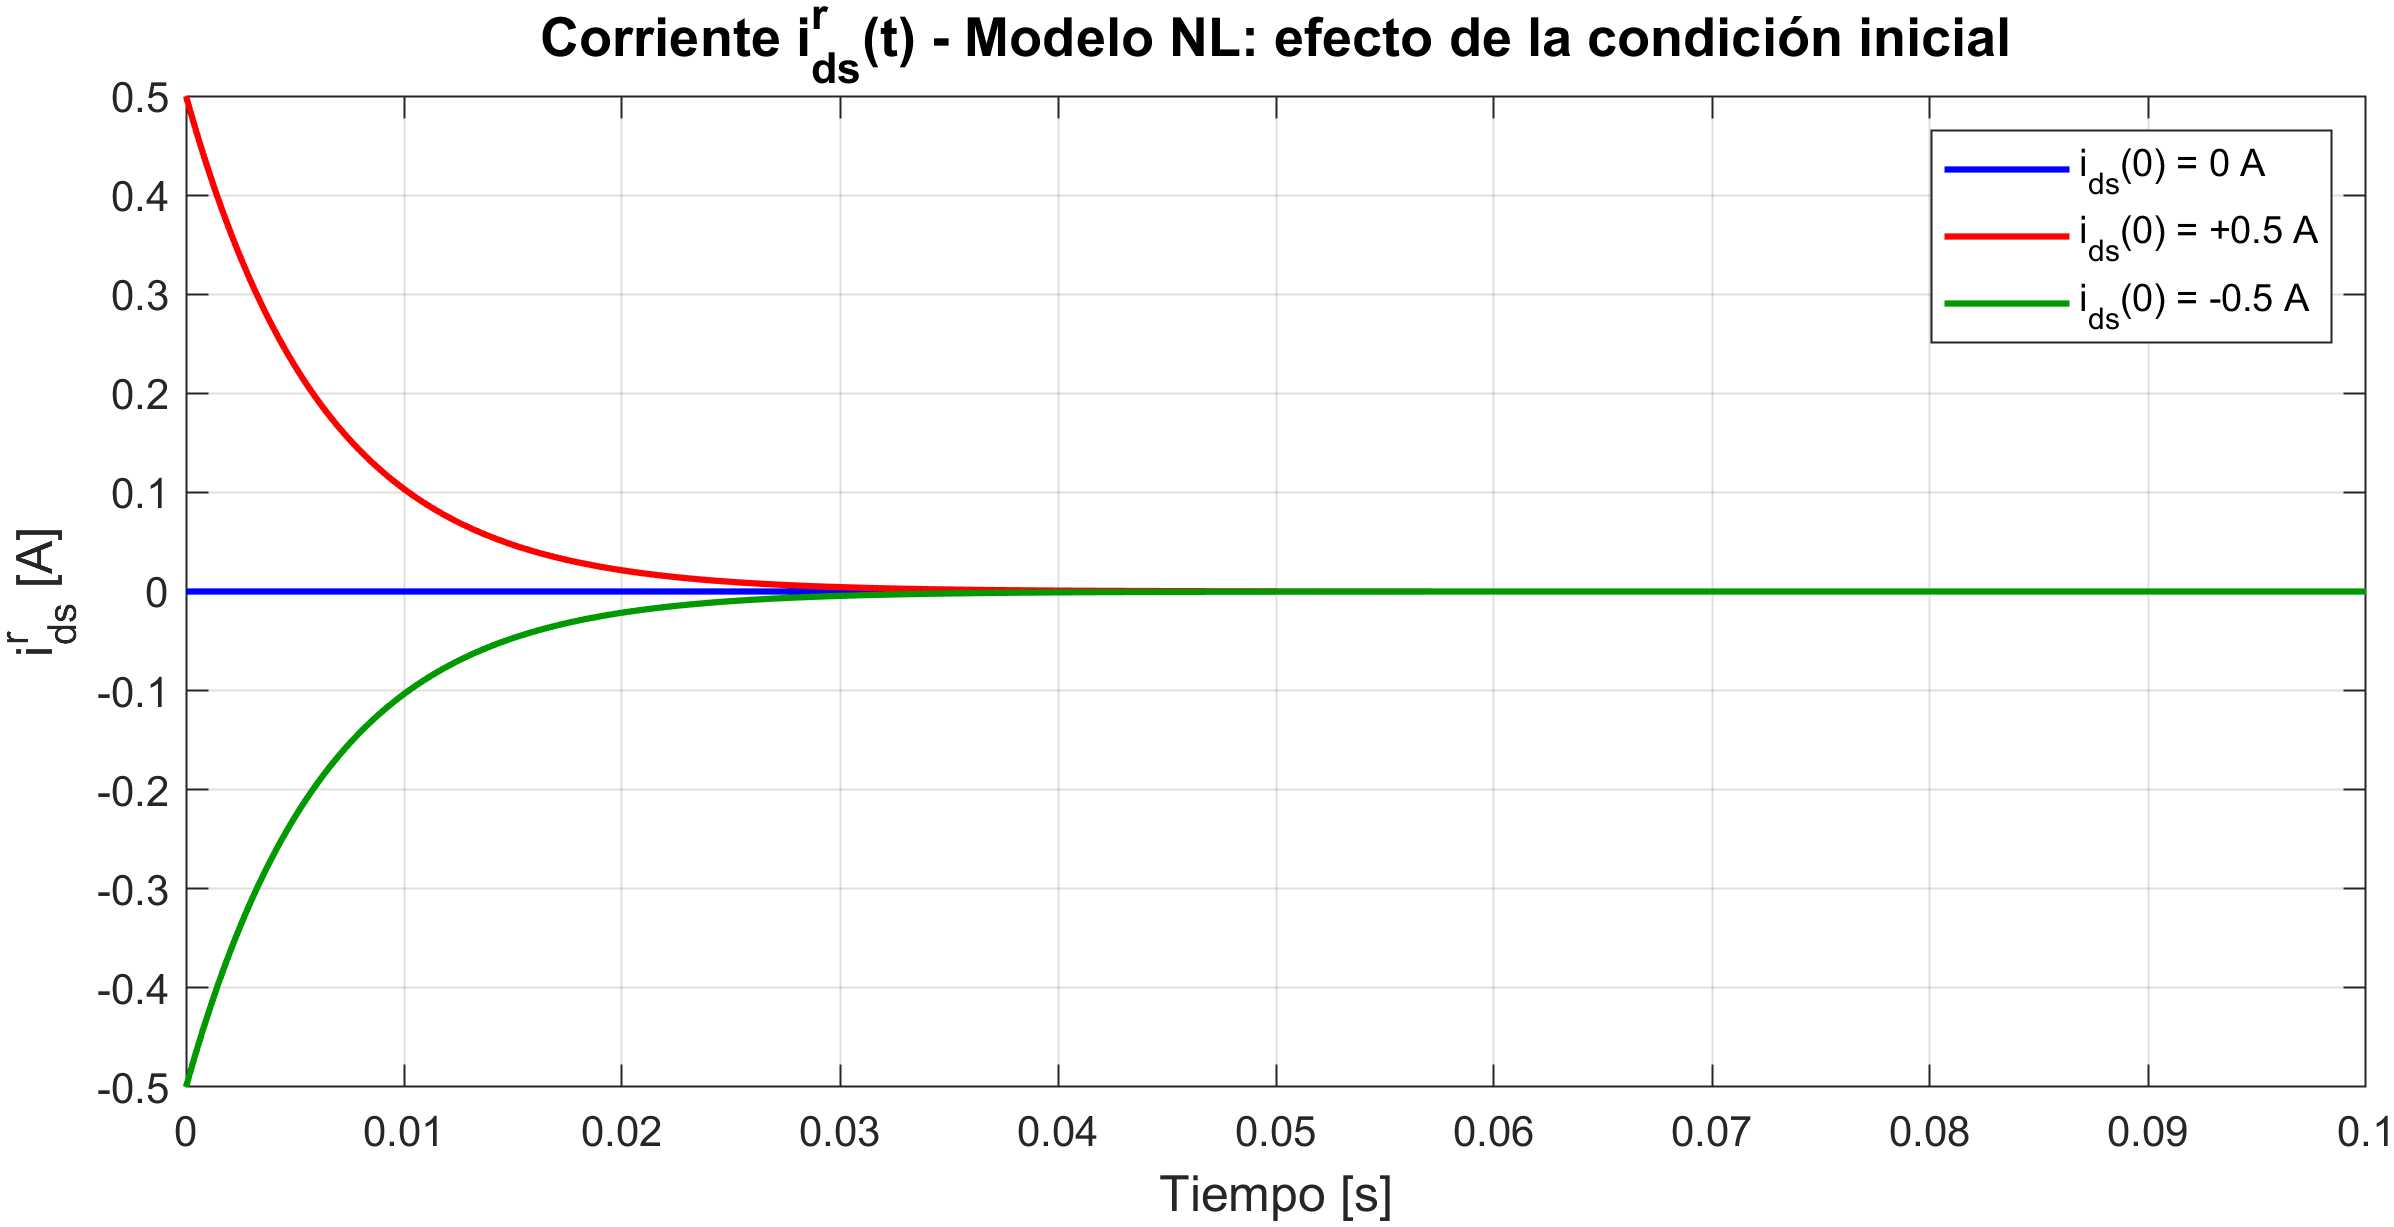
\includegraphics[width=0.9\textwidth]{imagenes/sim_ids_NL_3casos.png}
%    \caption{Comparación de $i_{ds}^r(t)$ para $i_{ds}^r(0) \in \{0,\; +0{,}5,\; -0{,}5\}$~A: modelo NL.}
%    \label{fig:sim_comparacion_ids}
%\end{figure}
%
%\begin{figure}[H]
%    \centering
%    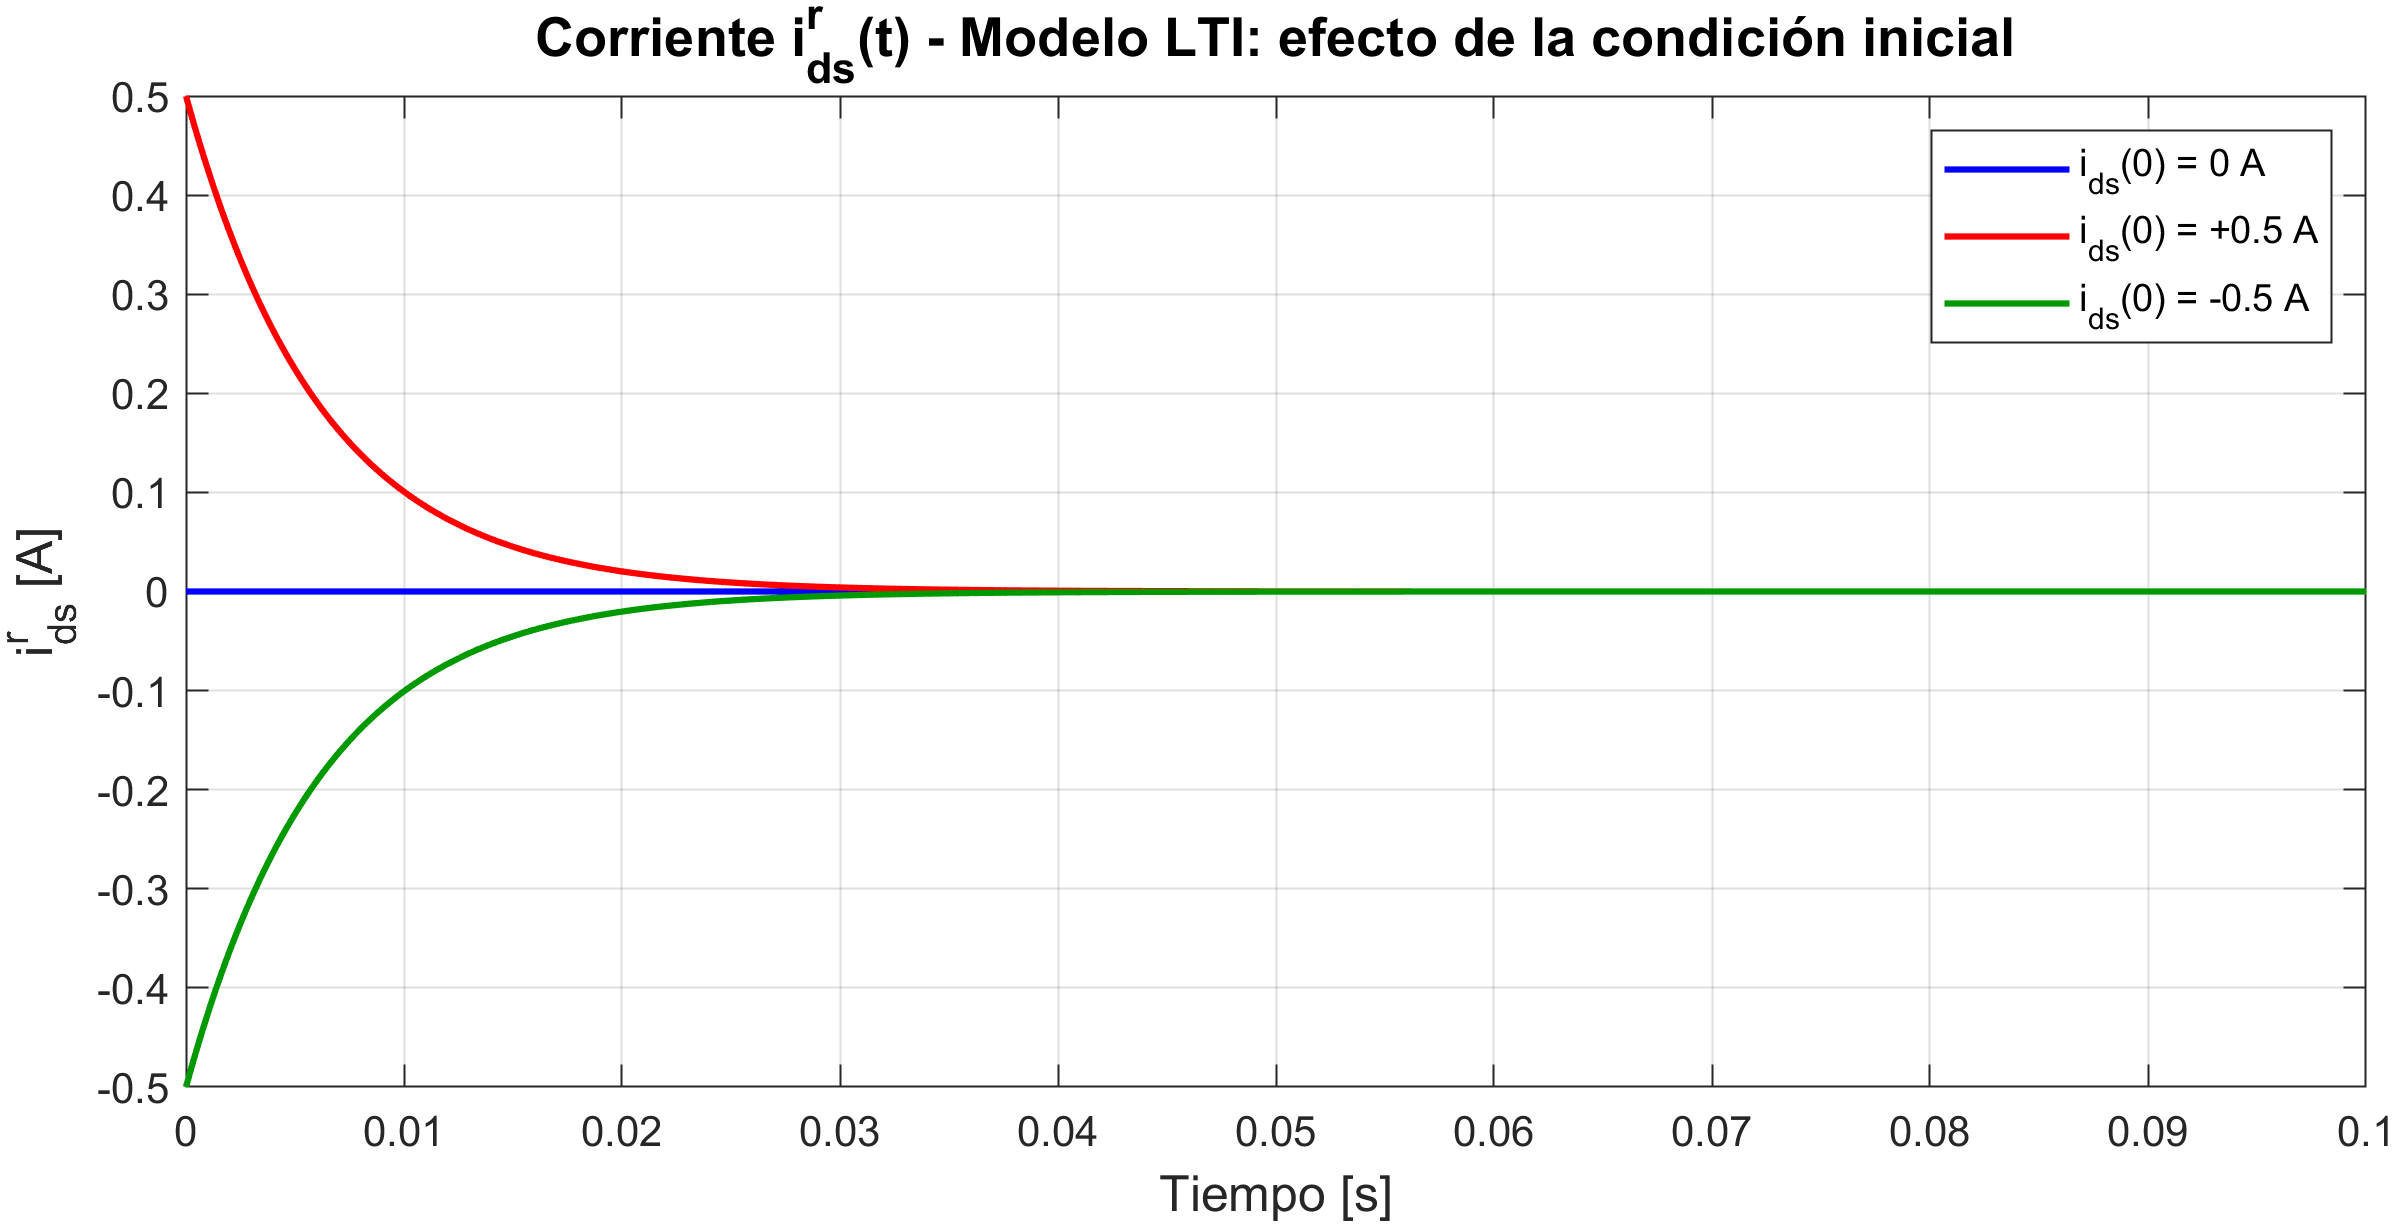
\includegraphics[width=0.9\textwidth]{imagenes/sim_ids_LTI_3casos.png}
%    \caption{Comparación de $i_{ds}^r(t)$ para $i_{ds}^r(0) \in \{0,\; +0{,}5,\; -0{,}5\}$~A: modelo LTI.}
%    \label{fig:sim_ids_zoom}
%\end{figure}

\textbf{Análisis:}
\begin{itemize}
    \item En el \textbf{modelo LTI}, $i_{ds}^r(t)$ decae como exponencial pura:
    \begin{equation}
        i_{ds}^r(t) = i_{ds}^r(0) \cdot e^{-t/\tau_d}, \quad \tau_d = \frac{L_d}{R_{s0}} = \frac{6{,}6 \times 10^{-3}}{1{,}02} = 6{,}47 \text{ ms}
    \end{equation}
    completamente \textbf{desacoplado} del resto de los estados. Esto es consecuencia de la estructura diagonal por bloques de la matriz $A_{aug}$: el polo $p_d = -R_{s0}/L_d \approx -154{,}5$~rad/s es real, estable y no comparte autovector con ningún otro estado.

    \item En el \textbf{modelo NL}, $i_{ds}^r(t)$ también decae exponencialmente con la misma constante de tiempo. Aunque existe un acoplamiento residual NL del tipo $\omega_r \cdot L_q \cdot i_{qs}$, la ley de control mínima ($v_{ds} = -L_q i_{qs} \omega_r$) lo cancela exactamente, y la ley complementaria ($v_{qs} = v_{qs}^* + \omega_r L_d i_{ds}^r$) elimina el efecto cruzado inverso.

    \item En ambos modelos, el efecto de $i_{ds}^r(0) \neq 0$ se extingue en $\approx 5\tau_d \approx 32$~ms, sin impacto apreciable sobre la dinámica mecánica ($\omega_m$, $\theta_m$) ni sobre $i_{qs}$. Esto justifica la hipótesis adoptada en la sección de linealización: la condición $i_{ds}^r(0) = 0$ no es restrictiva en la práctica, ya que cualquier valor inicial decae rápidamente a cero.
\end{itemize}

% =====================================================================
\subsubsection{Field Forcing y Field Weakening (Sub-ítem d)}
\label{sec:sim_item_d}

Se agrega una consigna de tensión en eje $d$, sumada a la ley de control mínima:
\begin{equation}
    v_{ds}(t) = \underbrace{-L_q \, i_{qs} \, \omega_r}_{\text{ley mínima}} + v_{ds}^*(t), \quad
    v_{ds}^*(t) = \begin{cases}
    0 & t < 0{,}5 \text{ s} \\
    +1{,}9596 \text{ V} & t \geq 0{,}5 \text{ s} \quad \text{(field forcing)}\\
    -1{,}9596 \text{ V} & t \geq 0{,}5 \text{ s} \quad \text{(field weakening)}
    \end{cases}
\end{equation}

donde $V_{ds}^* = V_{qs,nom}/10 = 1{,}9596$~V. Se simula con $i_{ds}^r(0) = 0$~A para aislar el efecto de la tensión inyectada.

% TODO Paso 3: descomentar cuando se tengan las imágenes de field forcing/weakening
%\begin{figure}[H]
%    \centering
%    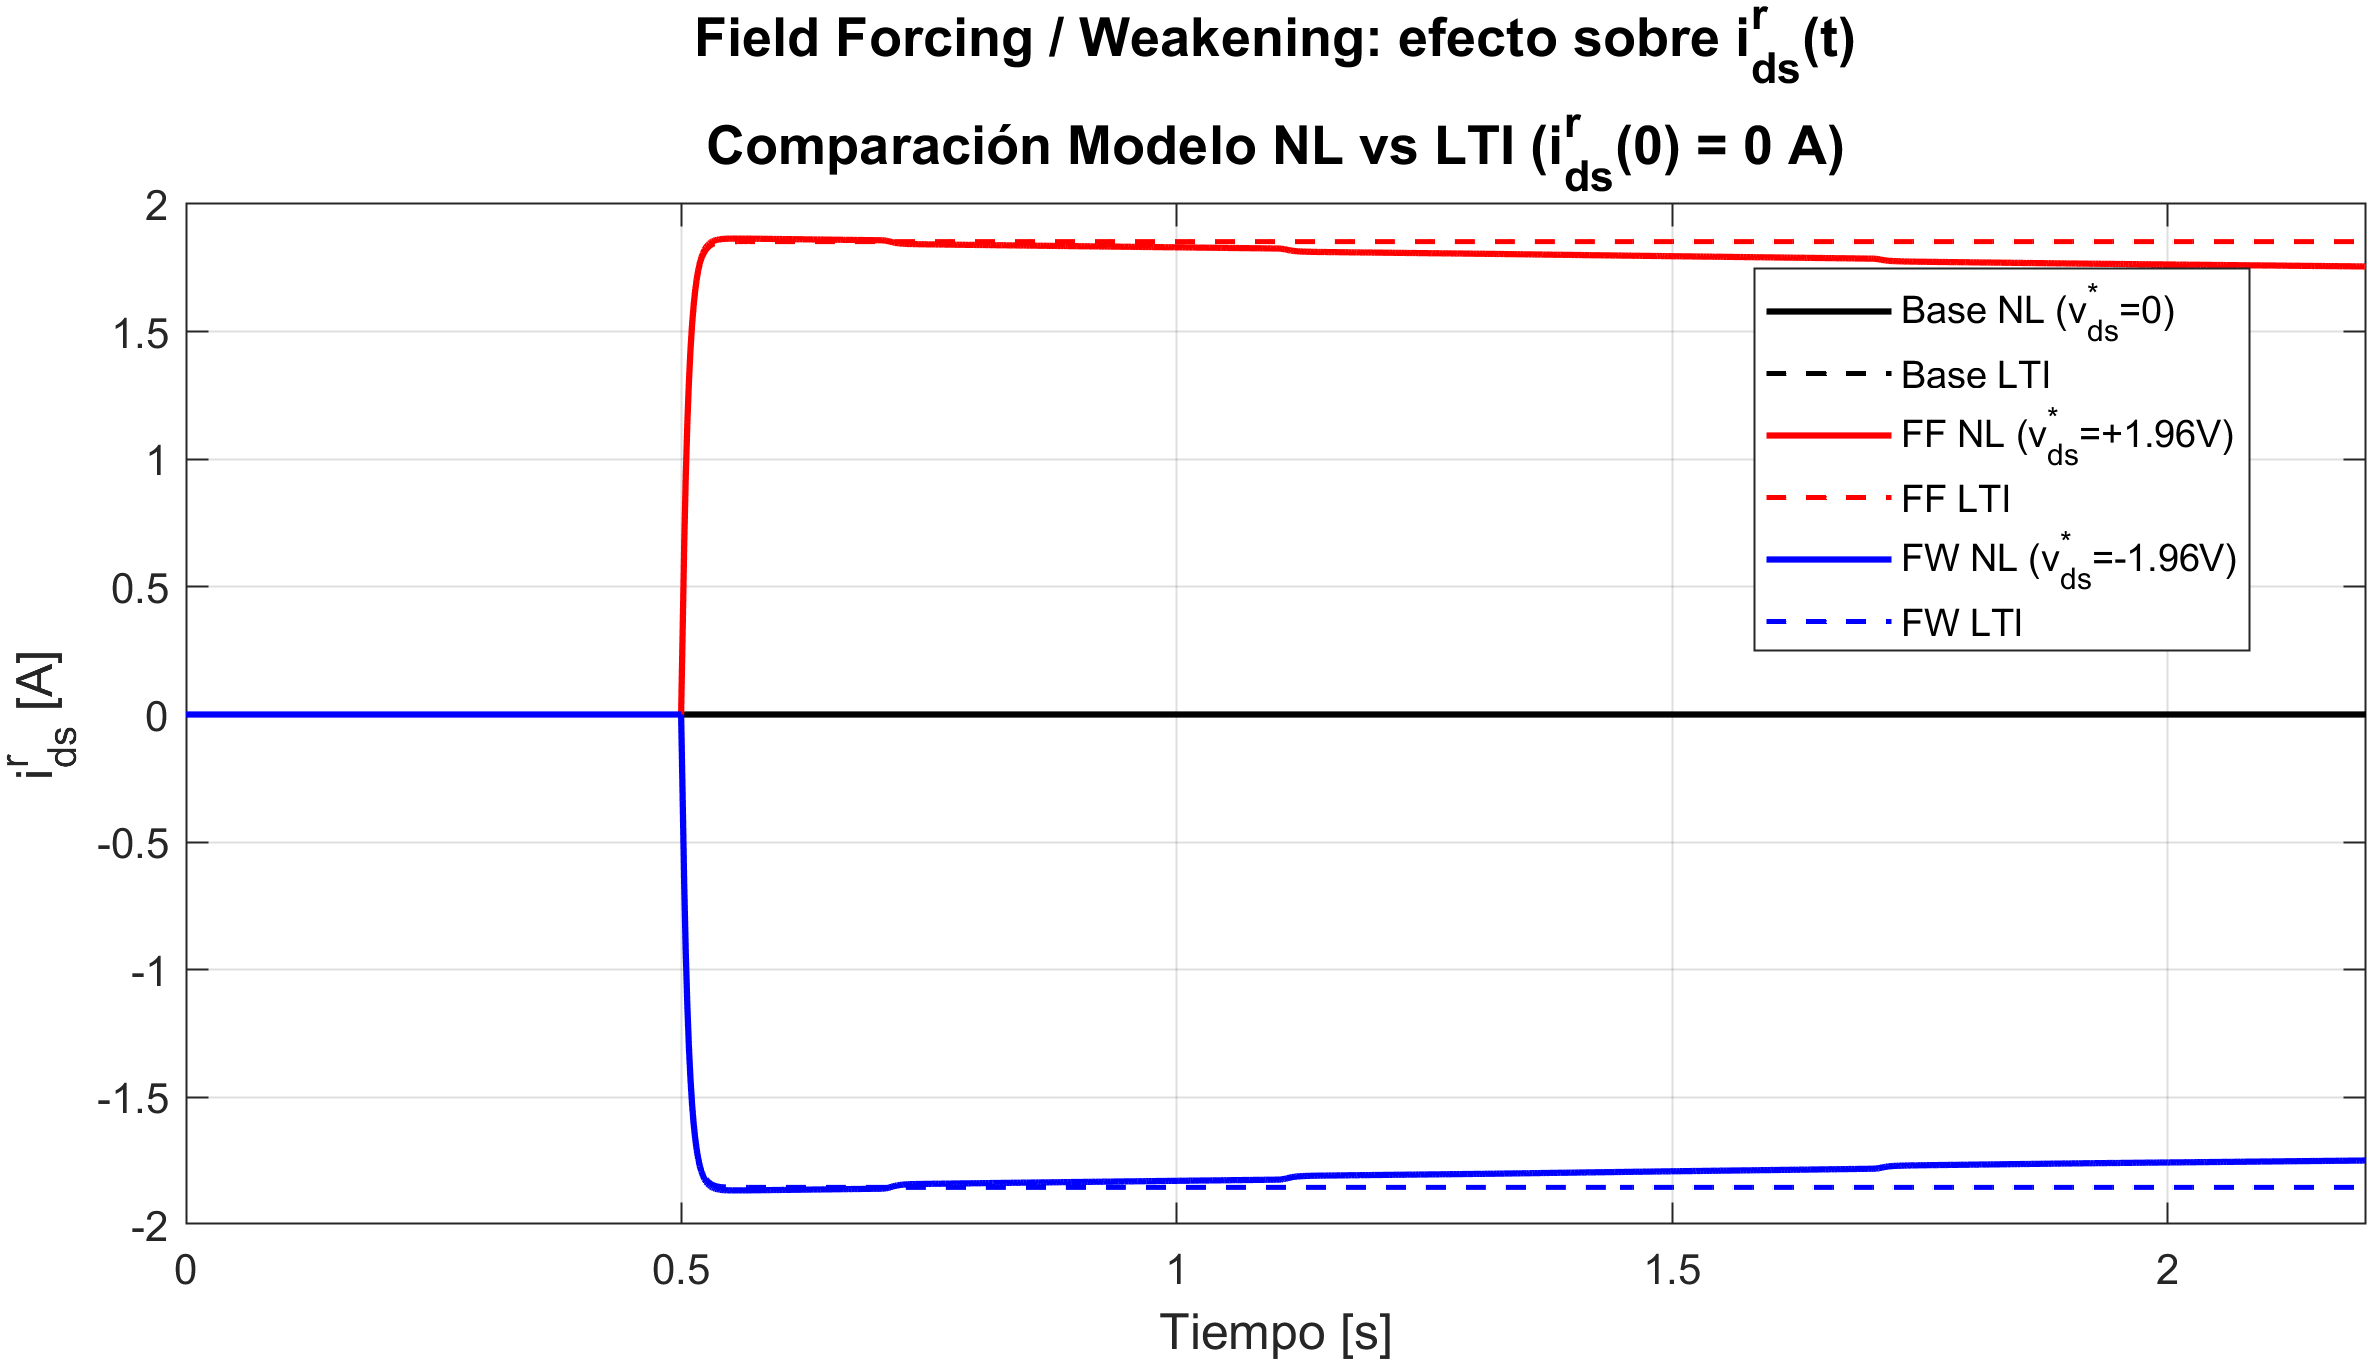
\includegraphics[width=\textwidth]{imagenes/sim_ff_ids.png}
%    \caption{Efecto del field forcing ($v_{ds}^* = +1{,}96$~V) y field weakening ($v_{ds}^* = -1{,}96$~V) sobre $i_{ds}^r(t)$, comparado con el caso base ($v_{ds}^* = 0$).}
%    \label{fig:sim_field_forcing}
%\end{figure}

\textbf{Análisis:}
\begin{itemize}
    \item En el \textbf{modelo LTI}, $v_{ds}^*$ afecta \textbf{únicamente} a $i_{ds}^r$, que crece exponencialmente hasta su valor estacionario $i_{ds,ss}^r = v_{ds}^*/R_{s0} = \pm 1{,}92$~A. Los demás estados ($\theta_m$, $\omega_m$, $i_{qs}$) permanecen \textbf{inalterados} por el desacoplamiento estructural de la matriz $A_{aug}$.

    \item En el \textbf{modelo NL}, $i_{ds}^r \neq 0$ introduce acoplamientos cruzados que el LTI no captura:
    \begin{itemize}
        \item \textit{Torque de reluctancia}: $\Delta T_m = \tfrac{3}{2}P_p(L_d - L_q) i_{ds}^r i_{qs}$, que modifica el torque electromagnético neto.
        \item \textit{FEM de acoplamiento}: los términos $\omega_r L_d i_{ds}^r$ en eje $q$ y $-\omega_r L_q i_{qs}$ en eje $d$ generan tensiones inducidas cruzadas.
    \end{itemize}

    \item Para \textbf{field forcing} ($v_{ds}^* > 0$): $i_{ds}^r > 0$ genera un torque de reluctancia positivo (dado que $L_d > L_q$) que incrementa el torque total, produciendo sobrepicos mayores en $\omega_m$ y un régimen estacionario levemente diferente.

    \item Para \textbf{field weakening} ($v_{ds}^* < 0$): el efecto es simétrico opuesto. La corriente $i_{ds}^r < 0$ debilita el campo magnético efectivo, reduciendo el torque disponible.

    \item Ambos efectos son pequeños para la amplitud utilizada ($V_{qs,nom}/10$), pero la diferencia entre modelos demuestra las \textbf{limitaciones del LTI}: al operar con $i_{ds}^r$ alejado de cero, los términos no lineales omitidos por la linealización se vuelven relevantes.
\end{itemize}
